\documentclass[10pt, a4paper]{article}

\usepackage[a4paper, top=0.5cm, bottom=0.5cm, left=0.5cm, right=0.5cm, landscape]{geometry}
\usepackage{mathtools}
\usepackage{amsfonts}
\usepackage{multicol}
\usepackage{setspace}
\usepackage{graphicx}
\usepackage[dvipsnames]{xcolor}



\author{Zachary Chua Yan Ern}
\date{22 September 2021}
\setstretch{1.25}

\newcommand{\highlight}[1]{{\color{red}\textbf{#1}}}
\newcommand{\blue}[1]{{\color{MidnightBlue}#1}}
\newcommand{\red}[1]{{\color{red}#1}}
\newcommand{\green}[1]{{\color{ForestGreen}#1}}
\newcommand{\tab}[0]{\hspace*{2mm}}

\begin{document}
	\scriptsize %tiny
	\setlength\parindent{0pt}
	\setlength{\columnseprule}{0.1pt}
	
	\begin{center}
		{\large CS2105 CheatSheet}\\
		by Zachary Chua
	\end{center}
	
	\begin{multicols*}{3}
		{\normalsize\textbf{Internet}}\\
		- The Internet is a network of connected computing devices\\
		- Devices are known as \highlight{hosts} or \highlight{end systems}\\
		- Hosts run network applications (like browsers) and communicate over links\\
		
		\textbf{Network Edge (Access Network)}\\
		- Hosts access the Internet through \highlight{access network}\\
		- eg Home/ Institute access networks\\
		
		\textbf{Wireless Access Network}\\
		1. Wireless LAN (WIFI): Short range (100 ft)\\
		2. Wide-area wireless access (3G/ 4G): Long range (10s km)\\	
		
		\textbf{Physical Media}\\
		Host connect to access network via physical media
		- Guided media: signals propogate in solid media (ethernet cable/ fibre optics)\\
		- Unguided media: signals propagate freely (radio)\\
		
		\textbf{Network Core}\\
		A mesh of interconnected routers\\
		Data transmitted by\\
		1. Circuit Switching: dedicated circuit per call\\
		2. Packet Switching: data sent through net in discrete "chunks"\\
		
		\textbf{Circuit Switching}\\
		End-to-end resources \highlight{allocated to and reserved for} "call" between source and dest\\
		- call setup required\\
		- circuit-like (\highlight{guaranteed}) performance\\
		- circuit segment idle if not used by call\\
		- used in traditional telephone networks\\
		- limited capacity\\
		
		\textbf{Packet Switching}\\
		Resources are used on demand $\rightarrow$ no reservation and excessive congestion is possible\\
		Performance not guaranteed\\
		Host sending function\\
		- breaks application message into smaller chunks, known as \highlight{packets} of length \highlight{L} bits\\
		- transmits packets onto the link at \highlight{transmission rate R}\\
		- link transmission rate is known as \highlight{link capacity} or \highlight{link bandwidth}\\
		
		Packet Transmission Delay = $\frac{L}{R}$, assuming packet size $L$ bits and link bandwidth $R$ bits/sec\\
		
		\highlight{Store and Forward}: entire packet must arrive at a router before it can be transmitted on the next link (check packet integrity; if corrupted, drop packet)\\
		
		\textbf{Routing and Addressing}\\
		Where to forward the packet\\
		- \red{Routers} determine the source-destination route taken by the packet (using routing algorithms)\\
		- \red{Addressing}: each packet needs to carry source and destination information\\

		\textbf{Delay and Loss}\\
		Loss:
		- Packets queue in router buffers - wait for turn to be sent out one by one\\
		- if packet arrival rate exceeds departure rate $\rightarrow$ buffer full and drop packet\\

		4 sources of delay\\

		1. Nodal Processing - check bit error, determine output link\\
		2. Queueing Delay - time waiting in queue for transmission\\
		3. Transmission Delay - $L/R$, where $L$ is packet length in bits, $R$ is link bandwidth in bps\\
		4. Propagation Delay - $d/s$, where $d$ is length of link, $s$ is propagation speed in medium\\

		\textbf{Throughput}\\
		How many bits can be transmitted per unit time\\
		- Measured for \red{end-to-end} commmunication\\
		- \red{Link capacity (bandwidth)} is meant for a \red{specific link}\\

		\textbf{Protocols}\\
		Defines \blue{format} and \blue{order} of messages exchanged and the \blue{actions} taken after messages are sent or received\\

		Internet Protocol\\
		1. Application - supports network applications\\
		2. Transport - process to process data transfer\\
		3. Network - routing of datagrams from source to destination\\
		4. Link - data transfer between neighbouring network elements\\
		5. Physical - bits on wire\\

		{\normalsize\textbf{Application Layer}}\\

		\textbf{Structure of Network Application}\\
		- Client-Server\\
		- Peer-to-peer\\

		\textbf{Client-Server}\\
		Server:\\
		- Wait for incoming request\\
		- Provides requested service to client\\
		Client:\\
		- Initiates contact with and request service from server\\

		\textbf{P2P}\\
		- No always on server\\
		- peer request service from other peers, provides service to other peers\\
		- self-scalable\\
		- complex management - peers are intermittently connected and change IP addresses\\

		\textbf{Transport Service does an app need}\\
		- Data Integrity\\
		- Throughput - Some apps may need minimum bandwidth (streaming videos)\\
		- Timing - might need low latency\\
		- Security - excryption\\

		\textbf{Transport Layer Protocol}\\
		App-layer protocols ride on transport layer protocols\\

		1. TCP\\
		- Reliable data\\
		- Flow Control: sender won't overwhelm receiver\\
		- Congestion Control: throttle sender when network overloaded\\
		- does not provide: \red{timing, minimum throughput, security}\\

		2. UDP\\
		- Unreliable data\\
		- no flow control\\
		- no congestion control\\
		- does not provide: timing, throughput, security\\

		\textbf{Web}\\
		Webpage typically consists of\\
		- base HTML file\\
		- several referenced objects\\
		Each object is addressable by a \red{URL}\\

		\textbf{HTTP - Web app layer protocol}\\
		C/S model\\
		- client in browser\\
		- server on port 80 (default port number for web servers)\\
		Uses TCP
		1. Client initiates TCP connection to server\\
		2. Server accepts TCP connection request\\
		3. HTTP Messages are exchanged over TCP connection\\
		4. TCP connection closed\\
		1 and 2 are known as \red{TCP handshaking}\\
		\red{RTT}: Round trup time, time for a packet to travel from client to server and go back.\\

		\textbf{Non-Persistent HTTP}\\
		- At most one object sent over TCP connection; TCP connection closed after object sent\\
		- downloading multiple objects requires multiple connections\\

		\textbf{Persistent HTTP}\\
		- multiple objects sent over single TCP connection between client and server\\

		(a): Non-persistent\\
		- $2 * RTT + $ file transmission time for each object (1 RTT for TCP, 1 RTT for object)\\
		(b): Non-persistent with pipelining\\
		- $2 * RTT + $ file transmission time for HTML page\\
		- as little as $2 * RTT + $ file transmission time for other objects (concurrently)\\
		(c): Persistent\\
		- 1 RTT for TCP\\
		- 1 RTT for each object\\
		(d): Persistent with pipelining\\
		- 1 RTT for TCP\\
		- 1 RTT for HTML\\
		- as little as 1 RTT for all referenced object\\

		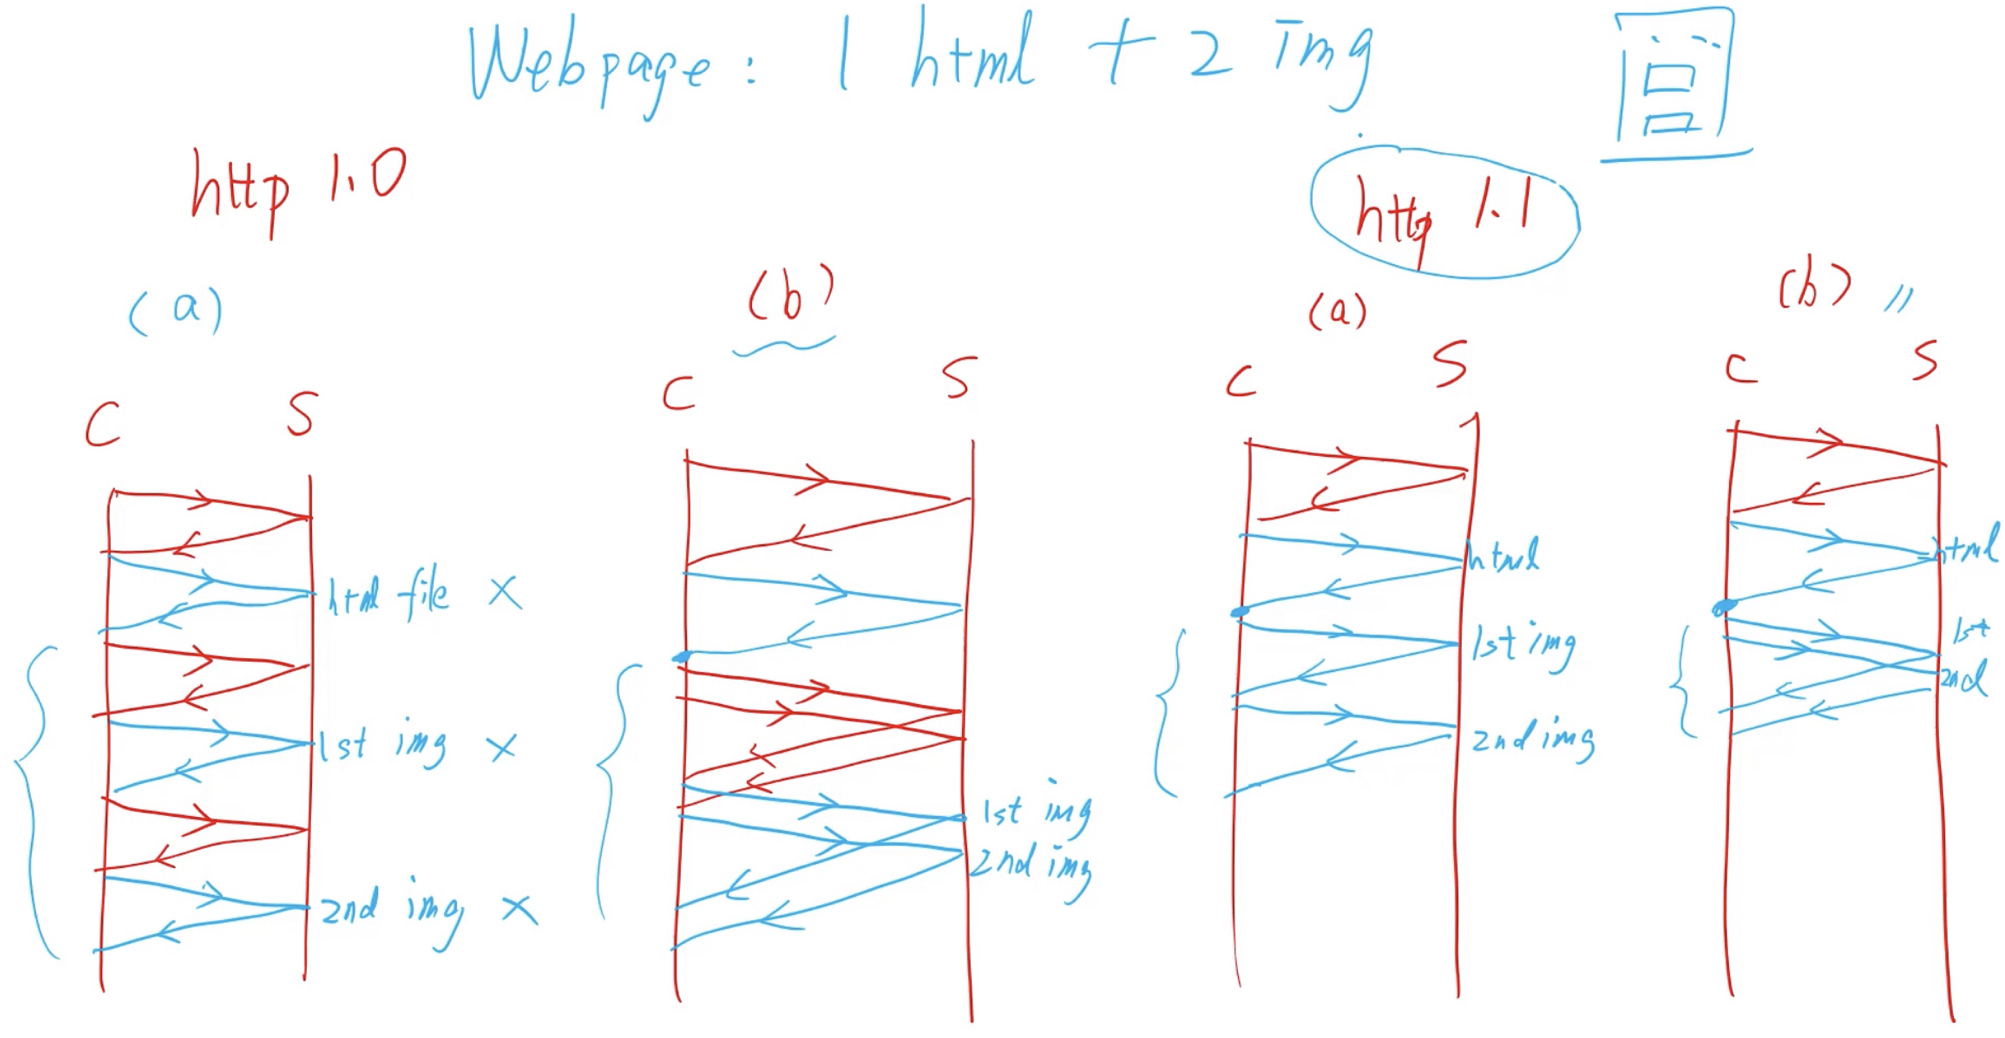
\includegraphics[scale=.12]{./assets/httpDiagrams}

		\textbf{HTTP Request}\\
		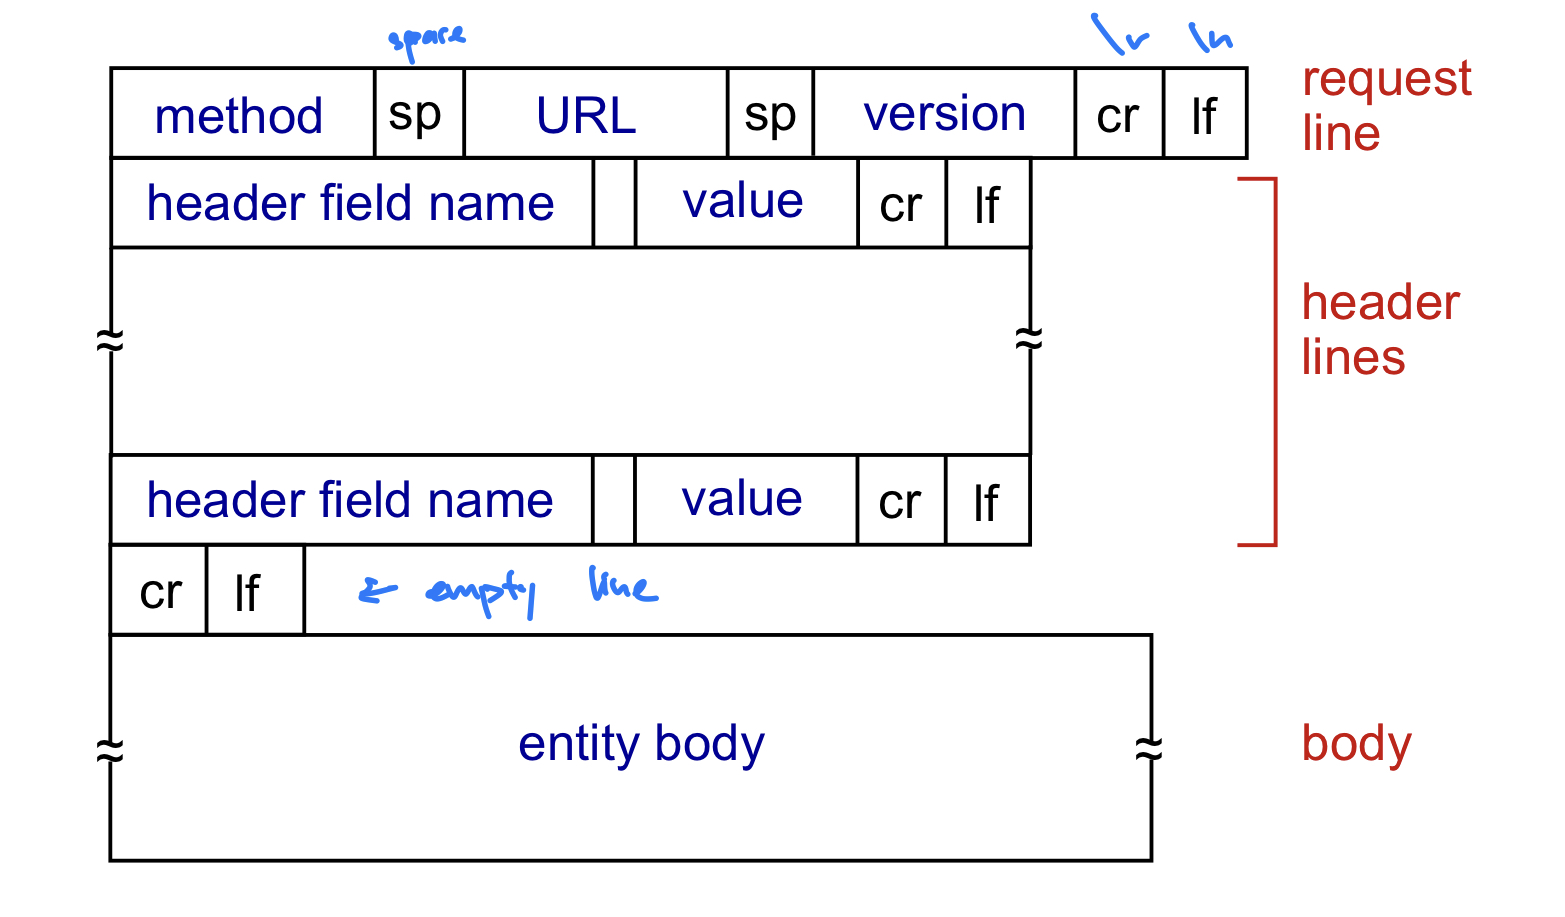
\includegraphics[scale=.14]{./assets/httpRequest}
		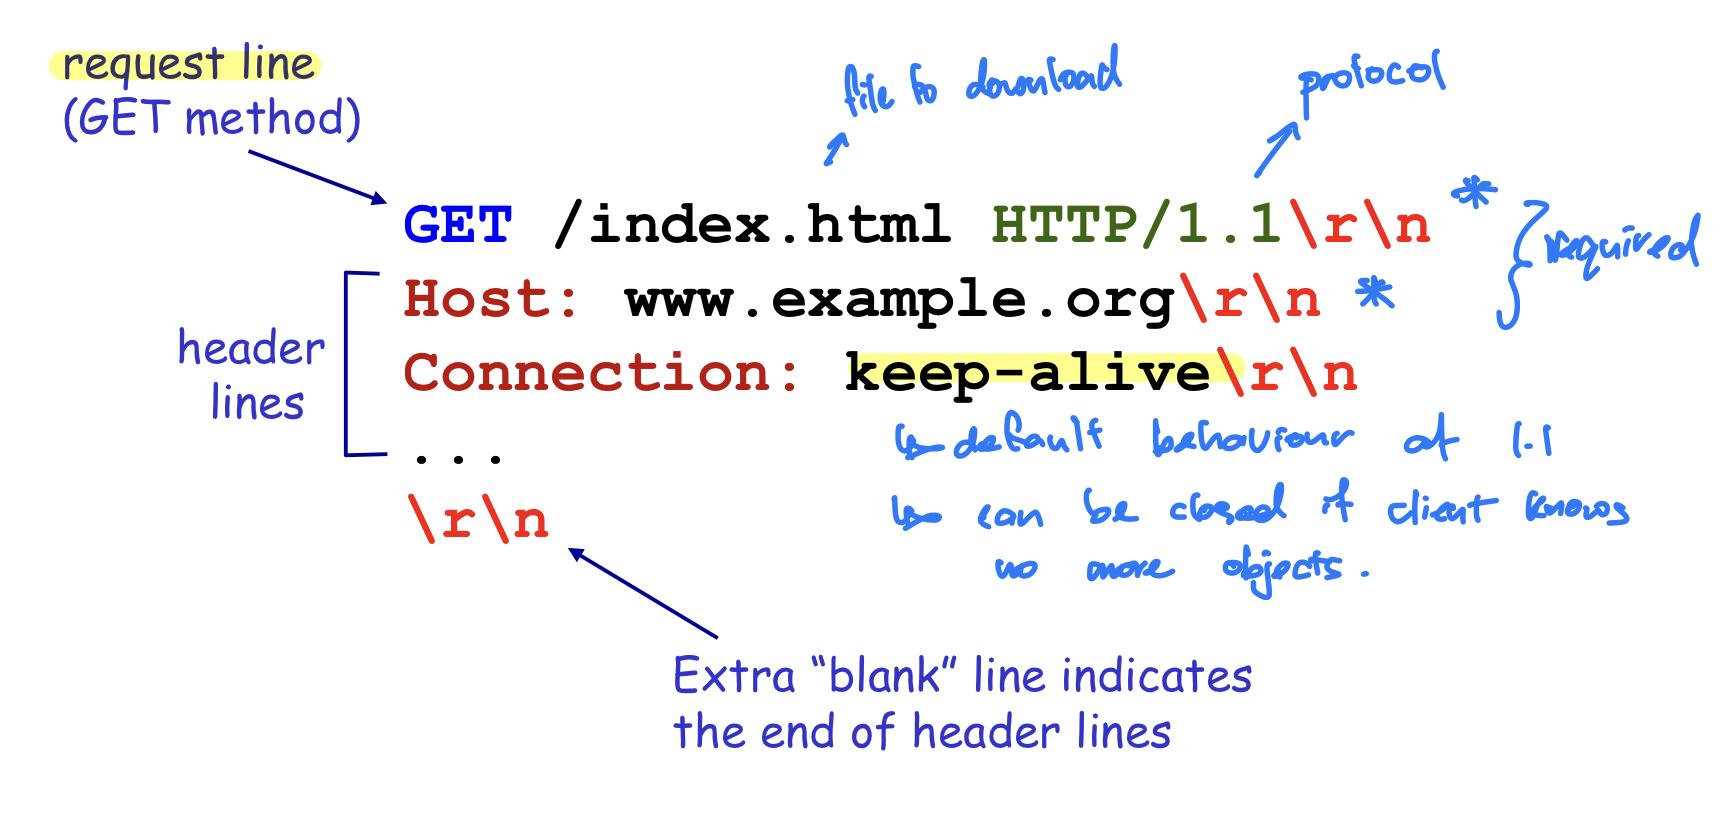
\includegraphics[scale=.12]{./assets/httpRequestEg}\\
		Request Method Types:\\
		1.0: GET, POST (upload input to server), HEAD (leave out requested object)\\
		1.1: GET, POST, HEAD, PUT (uploads file to path specified in URL field), DELETE (deletes file specified in URL field)\\

		\textbf{HTTP Response}\\
		Response Status Codes:\\
		- 200: OK\\
		- 301: Moved Permanently (new location specified later in message)\\
		- 403: Fobidden\\
		- 404: Not found\\
		- 304: Not Modified\\
		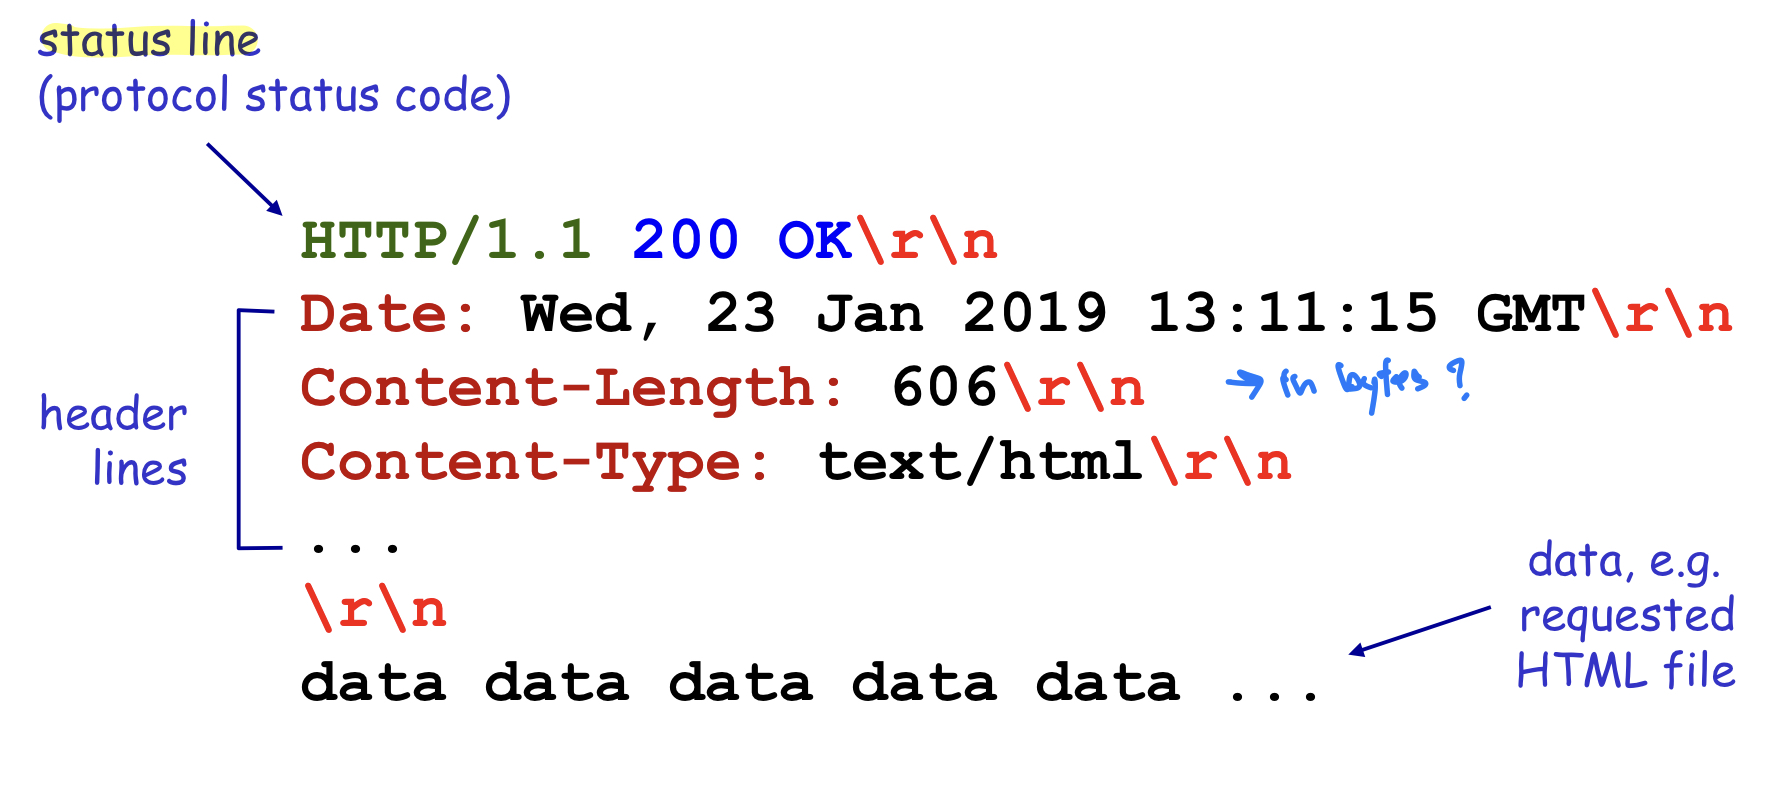
\includegraphics[scale=.12]{./assets/httpResponseEg}

		\textbf{Cookies}\\
		HTTP designed to be stateless - server maintains no information about past client requests\\
		Cookie: http messages carry state (forever, expiry, memory only)\\
		1. cookie header field of http request/ response messages\\
		2. cookie file kept on user's host, managed by user's browser\\
		3. backend database at website\\

		\textbf{Conditional Get}\\
		- Goal: don't send object if client cache has up to date cached version\\
		- cache: specify date of cached copy in http request; \texttt{If-modified-since: <date>}\\
		- server: response contains no object if cached copy is up to date; response is 304\\

		\textbf{Domain Name System}\\
		Identify host by:
		1. Hostname: eg, www.example.org\\
		2. IP address: eg, 93.184.216.34 (32-bit int)\\
		DNS translates between the two\\
		Client carries out DNS query to determine the IP address corresponding to server name prior to connection\\
		\red{NOTE}: 1 hostname could map to many IP addresses (for load balancing purposes)\\

		\textbf{DNS Resource Record (RR)}\\
		Mappings are stored as RR\\
		RR format: \texttt{(name, value, type, ttl)}\\

		Types:
		1. A - name is hostname; value is IP addr\\
		2. NS (name server) -name is domain (eg. nus.edu.sg); value is hostname of authoritative name server for domain.\\
		3. CNAME - name is alias name (eg. www.nus.edu.sg) for some canonical (real) name; value is canonical name (eg. mgnzsqc.x.incapdns.net)\\
		4. MX (mail exchanger) - value is the name of mail server associated with name\\

		\textbf{Distributed Hierarchical Databases}\\
		DNS is stored in RR in distributed databases implemented in hierarchy of many name servers\\
		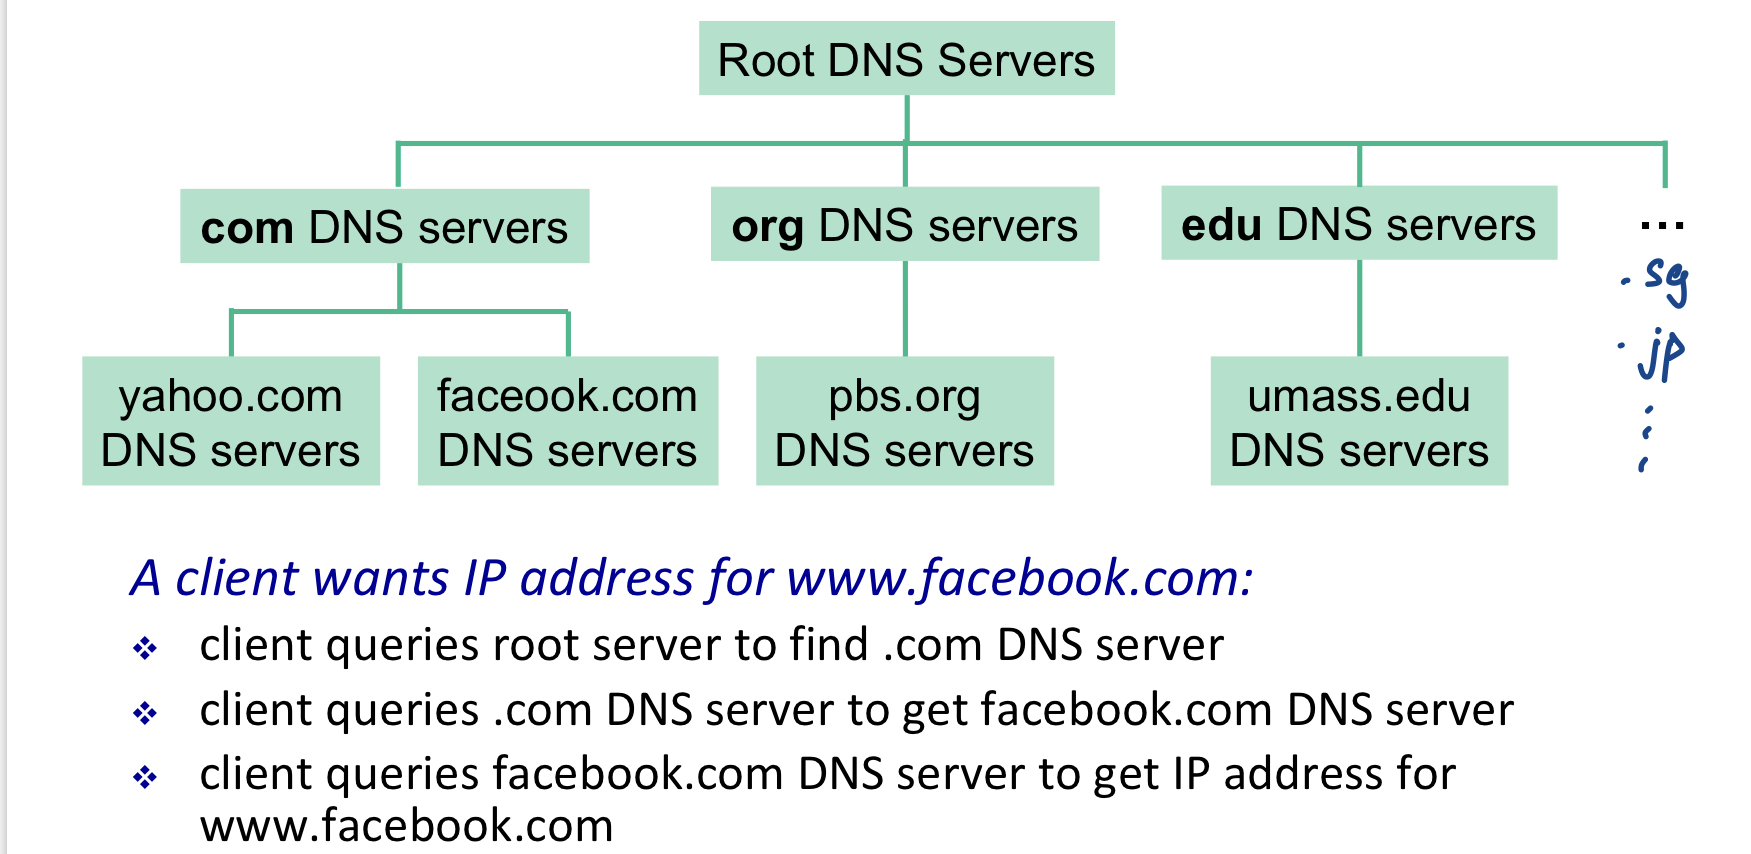
\includegraphics[scale=.13]{./assets/dnsDatabases}

		Root servers\\
		- Answers request for records in the root zone by returning a list of the authoritative NS for the appropriate top level domain (TLD)\\

		Top Level Domain\\
		- responsible for com, org, net, edu, etc and all top-level country domains, eg. sg, jp, etc.\\

		Authoritative Servers\\
		- Organisation's own DNS server(s), providing authoritative hostname to IP mappings for organisation's named hosts (eg. web, mail)\\

		\textbf{Local DNS server}\\
		- Does not strictly belong to hierarchy\\
		- Each ISP has one local DNS server (aka default name server)\\
		- When host makes DNS query, query is sent to local DNS server\\
		- Retrieve name-to-address translation from local cache\\
		- Local DNS server acts as proxy and forwards query into hierarchy if answer not found locally\\

		\textbf{DNS Caching}\\
		Caches mapping once it learns of it\\
		- may be out of date\\
		- cached entries expire after some time (TTL)\\
		- if name host changes IP address, may not be known Internet-wide until TTL expire\\
		Runs over \red{UDP}\\

		\textbf{DNS name resolution}\\
		iterative and recursive\\
		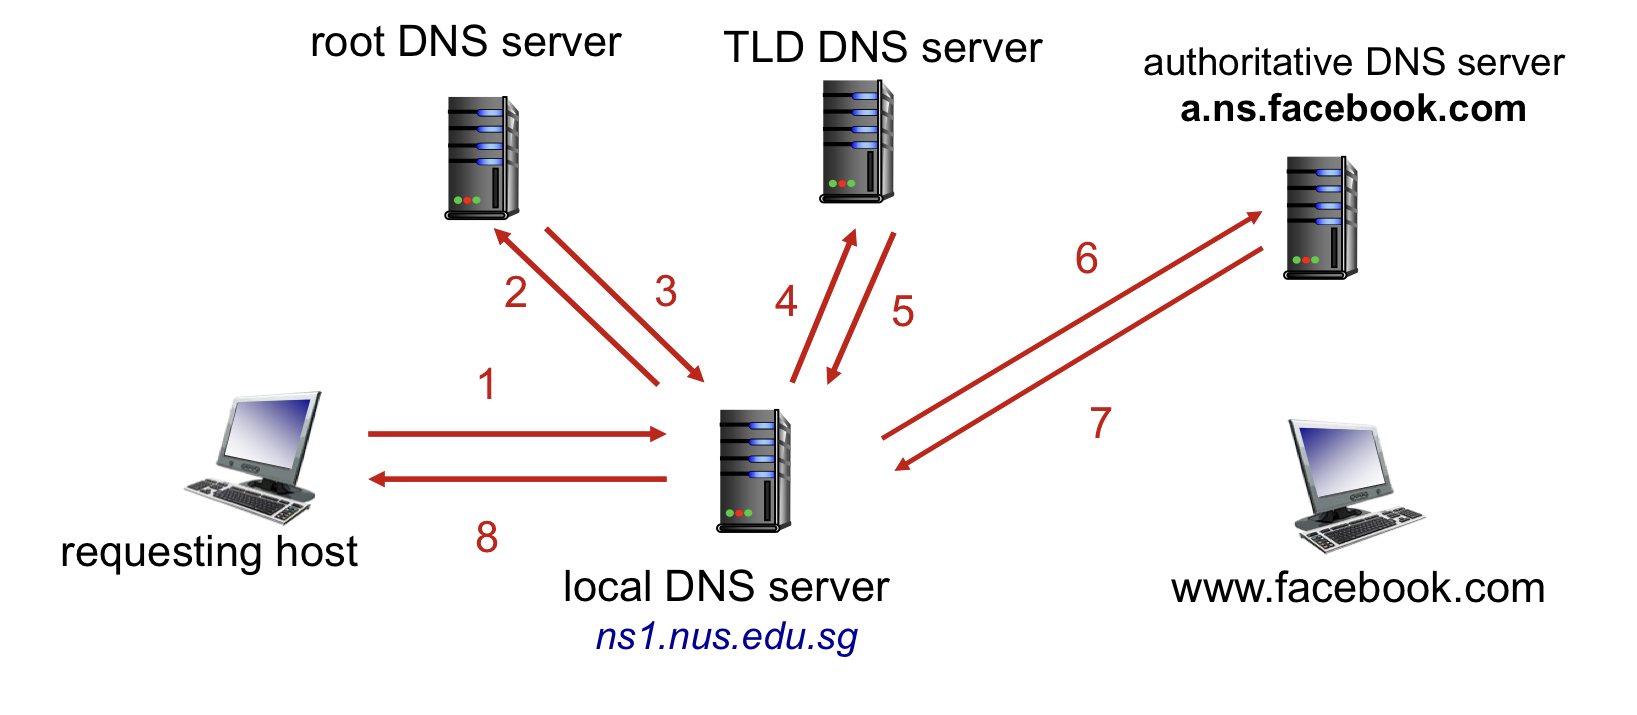
\includegraphics[scale=.12]{./assets/iterativeDns}\\
		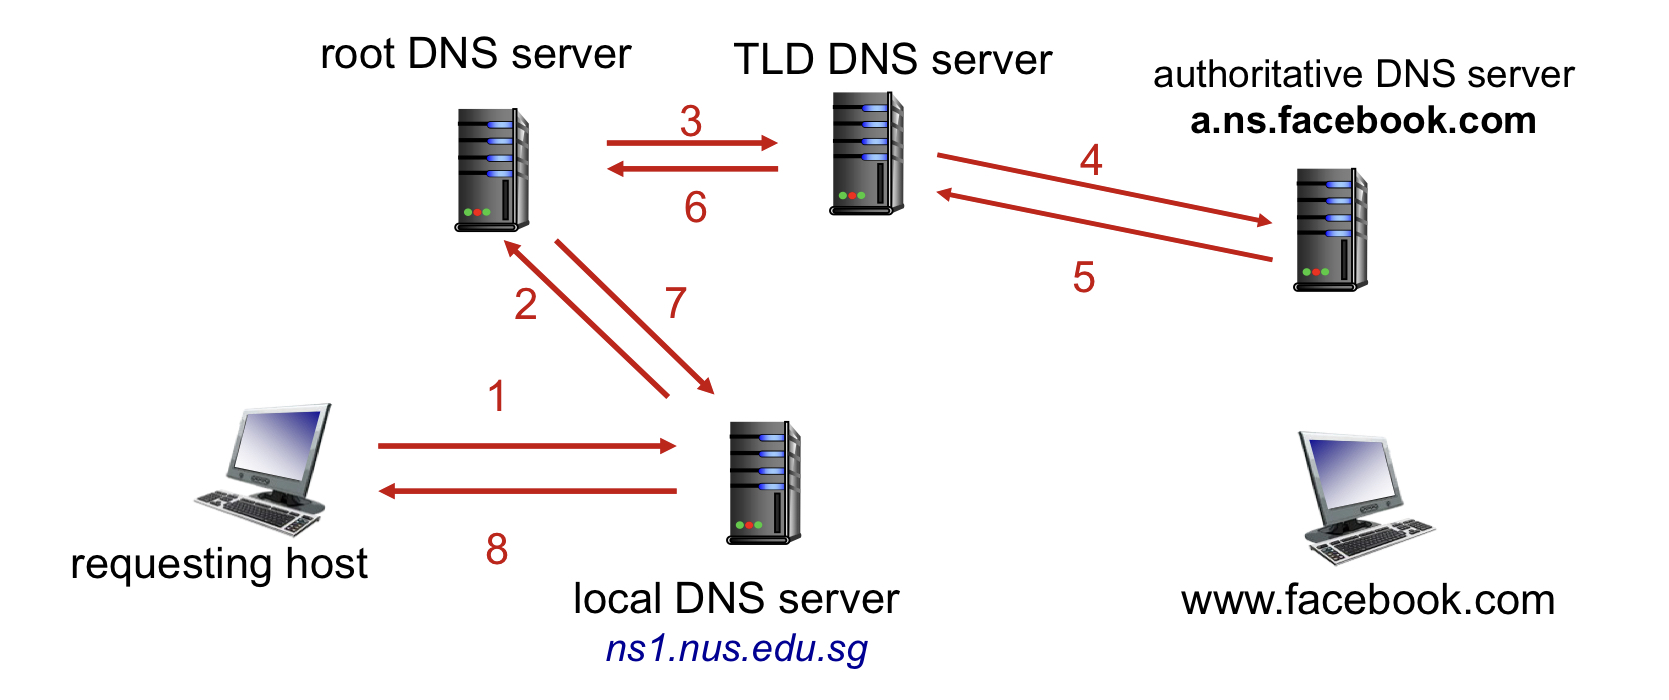
\includegraphics[scale=.12]{./assets/recursiveDns}\\
		\red{NOTE}: Recursive rarely used as servers cannot respond to other queries until it recieves an answer, eg root DNS cannot answer other queries until TLD server replies\\

		\textbf{Socket Programming}\\
		Process: program running within a host\\
		- Within host, two processes communicate using \red{inter-process communication (defined by OS)}\\
		- Processes in different hosts communicate by \red{exchanging messages (according to protocols)}\\
		- Identified by \red{(IP address, port number)} (port number is a 16 bit int, 1-1023 are reserved)\\

		\textbf{Sockets}\\
		Socket is the software interfrace between app processes and transport layer protocols
		- Process send/ receives messages to/ from its \red{socket}\\
		- Programming-wise: a set of APIs\\
		Application treat the Internet as a black box, sending and receiving messages through sockets\\

		Types of sockets:\\
		1. TCP: reliable, byte stream-oriented socket\\
		2. UDP: unreliable datagram socket\\

		\textbf{Socket Programming with \red{UDP}}\\
		\red{UDP: no connection between client and server}\\
		- Sender explicitly attaches destination IP addr and port number to \red{each packet}\\
		- Receiver extracts sender IP addr and port number from the received packet\\
		\red{1} socket listens to \red{multiple} clients.\\

		\textbf{Socket Programming with \red{TCP}}\\
		- When client creates socket, client TCP establishes a connection to server TCP\\
		- When contacted by client, server TCP \red{creates} new socket for server process to communicate with that client\\
		This allows server to talk with multiple clients individually.\\
		TCP socket pairs (?) are uniquely identified by \blue{(server IP, server port, client IP, client port)}\\

		TCP socket vs UDP socket\\
		- TCP: two processes communicate as if there is a ``pipe'' between them. Send data $\rightarrow$ write data to pipe, \blue{no need to attach} dest IP and port to each packet. Pipe is there until one of the two processes closes it. Pipe is also \blue{reliable}\\
		- UDP: Form UDP packet explicitly and \blue{attach} dest IP and port no to every packet.\\

		{\normalsize\textbf{Transport Layer}}\\
		Deliver messages between application processes running on different hosts\\
		- \blue{TCP} and \blue{UDP}\\

		What do they do\\
		- Sender: break app message into \blue{segments}, passes them to network (IP) layer\\
		- Receiver: reassembles segments into message, passes to app layer\\
		- Routers in between: check dest IP to determine routing\\

		Note:
		- Each IP datagram contains \blue{source and dest IP addr}\\
		- Each IP datagram carries \blue{one transport layer segment}\\
		- Each segment contains \blue{src and dest port numbers}\\

		\textbf{Connectionless Transport: UDP}\\
		UDP adds the following services (very few)\\
		- \blue{Multiplexing} at sender: UDP gathers data from processes, forms packets and passes them to IP\\
		- \blue{De-multiplexing} at receiver: UDP receives packets from lower layer and sends them to right processes\\
		- \blue{Checksum}\\
		\red{NOTE}: UDP transmission is \highlight{unreliable}\\
		Reasons for UDP:\\
		- No connection establishment (less delay)\\
		- Simple: no connection state at sender, receiver\\
		- small header size\\
		- No congestion control: UDP can blast away as fast as desired\\

		\textbf{Connectionless Demultiplexing}\\
		When UDP \red{receiver} recieves UDP segment\\
		- Checks \blue{dest port no} of segment\\
		- Directs UDP segment to the socket with that port number\\
		- IP datagrams (from different soucres) with \blue{same destination port no.} will be directed to the same UDP socket at destination\\

		\textbf{UDP Header}\\
		Comprises of (8 bytes / 64 bits)\\
		- Source port no. (16)\\
		- Dest port no. (16)\\
		- length \red{in bytes, including header}(16)\\
		- checksum (16)\\

		\textbf{UDP Checksum}\\
		To detect errors (flipped bits) in transmitted segment\\

		Sender:\\
		- Compute checksum value\\
		- put checksum value in UDP checksum field\\
		Receiver:\\
		- Compute checksum of received segment\\
		- Check if computed value = checksum\\
		\highlight{NOTE:} Just because checksum = computed value \red{does not} mean that there is no error\\

		Computation:\\
		1. Treat segment as a sequence of \blue{16-bit} integers\\
		2. Apply binary addition on every 16 bit integer (checksum field is currently 0)\\
		3. Carry (if any) from the MSB will be added to the result\\
		4. Compute 1s complement to get UDP checksum\\

		\textbf{Reliable Data Transfer}\\
		Network layer is \red{unreliable}, need to build reliable data transfer over this\\
		Network layer may:\\
		- corrupt, drop, re-order (not considered in this mod) packets, and deliver packets after an arbitrarily long delay\\

		rdt 2.0: \red{Bit Errors}\\
		\green{Solution:} Use checksum to detect bit errors, receiver replies with \blue{ACK/NAK} to acknowledge/ negative acknowledge\\
		- ACK: send next packet\\
		- NAK: resend current packet\\
		\red{Problem:} ACK may be corrupted. Sender would resend packet, receiver does not know it is duplicate\\

		rdt 2.1: \red{Bit Errors}\\
		\green{Solution:} rdt 2.0 with packet sequence number\\
		- ACK/NAK corrupted: Sender retransmits current packet\\
		- Sender adds sequence number to each packet.\\
		- Receiver discards (doesnt deliver to application) duplicate packets.\\

		rdt 2.0: \red{Bit Errors}\\
		\green{Modification}: NAK free. Receiver sends ACK for \blue{last packet received OK}. ACK now contains seq no.\\
		Duplicate ACK: resend \blue{current packet}\\

		rdt 3.0: \red{Errors and Loss}\\
		Channel may now:\\
		- flip bits\\
		- lose packets\\
		- arbitrarily long delay between packets\\
		- but \red{WON'T} reorder packets\\
		\green{Solution:} Sender waits for some time for ACK. Sender \blue{retransmits} if no ACK is received till \blue{timeout}\\
		\highlight{NOTE:} If packet or ACK is just delayed not lost;\\
		- Timeout triggers retransmission\\
		- Retransmission generates \blue{duplicates}, receiver uses seq no to detect\\
		- Reciever must specify the packet seq no of the packet being ACKed\\
		\red{NOTE:} Sender does not retransmit on ACK with \red{wrong packet no.} (just waits for timeout)\\

		\textbf{Performance of rdt 3.0 (bad)}\\
		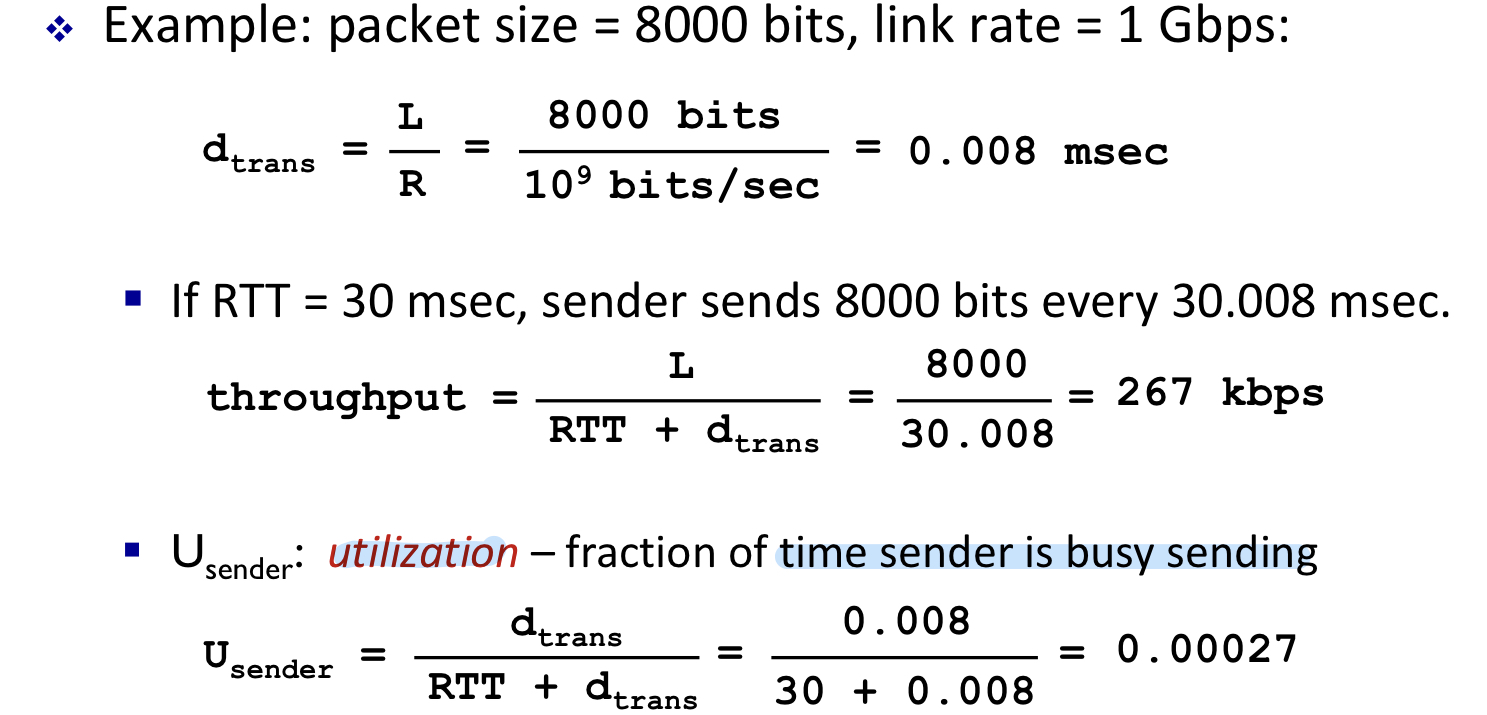
\includegraphics[scale=.145]{./assets/rdtPerformance}

		\textbf{Pipelined Protocols}\\
		Allows \blue{multiple, yet-to-be-ACKed} packets\\
		Requires more seq no, and buffering at both sides\\
		2 generic forms:\\
		- Go-Back-N (GBN)\\
		- Selective Repeat (SR)\\
		Same assumptions as rdt 3.0\\

		\textbf{GBN}\\
		GBN Sender:\\
		- Can have up to \blue{N unACKed packets} in pipeline\\
		- insert k-bits seq no in packet header\\
		- use ``sliding window'' to keep track of unACKed packets\\
		- keep a \blue{timer} for the \blue{oldest} unACKed packet\\
		- on timeout, retransmit all packets in sender window\\
		- \texttt{timeout(n)}: retransmit packet n and all subsequent packets in the window\\

		GBN Receiver:\\
		- \blue{In order packets}: ACK (simple receiver - only needs to keep track of the next expected seq no)\\
		- \blue{Out of order packets}: Discard and ACK the \blue{last in order packet}\\
		- \red{Cumulative ACK:} \texttt{ACK m} means all packets up to m are received\\

		\textbf{SR}\\
		SR Sender:\\
		- maintains timer for each unACKed packet\\
		- When timer expires, just retransmit \blue{only that unACKed packet}\\

		SR Receiver:\\
		- \red{Individually acknowledges} all correctly received packets\\
		- \blue{buffers out of order packets}, as needed, for eventual in-order delivery to upper layer\\
		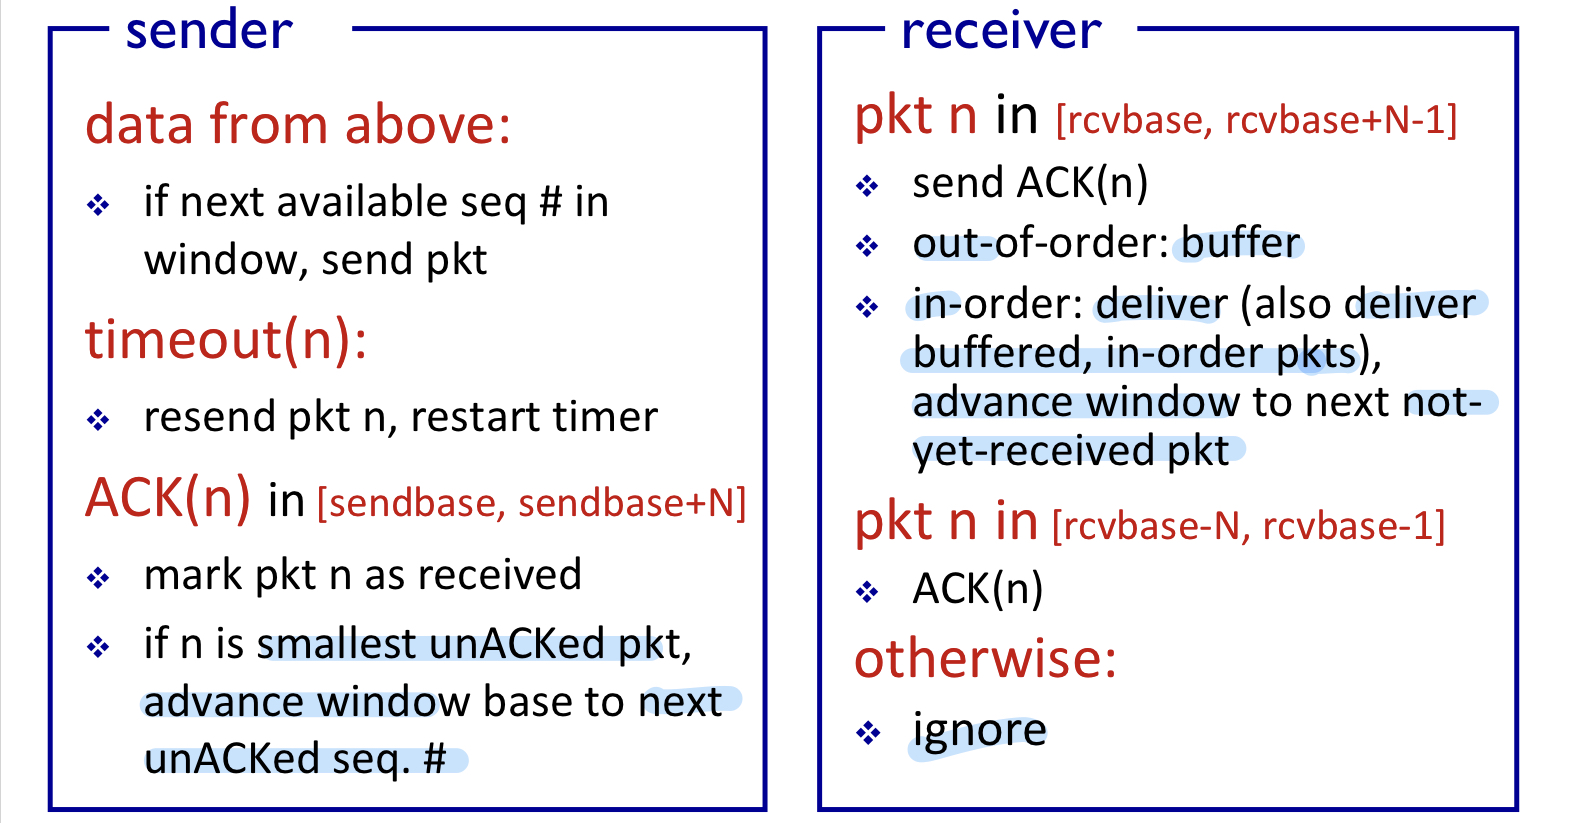
\includegraphics[scale=.14]{./assets/selectiveRepeat}

		\textbf{TCP}\\
		Overview:\\
		- Point-to-Point: 1 sender, 1 receiver\\
		- Connection-oriented: handshaking before sending app data\\
		- Full duplex service: bi-directional data flow in the same connection\\
		- Reliable, in-order byte stream: use seq no. to label bytes\\

		Connection Oriented De-mux:\\
		A TCP connection socket is identified by the 4-tuple (srcIP, srcPort, destIP, destPort)\\

		Segment Size:\\
		A TCP segment typically has an MSS (maximum segment size) of 1460 bytes (app data, without header)\\

		Header:\\
		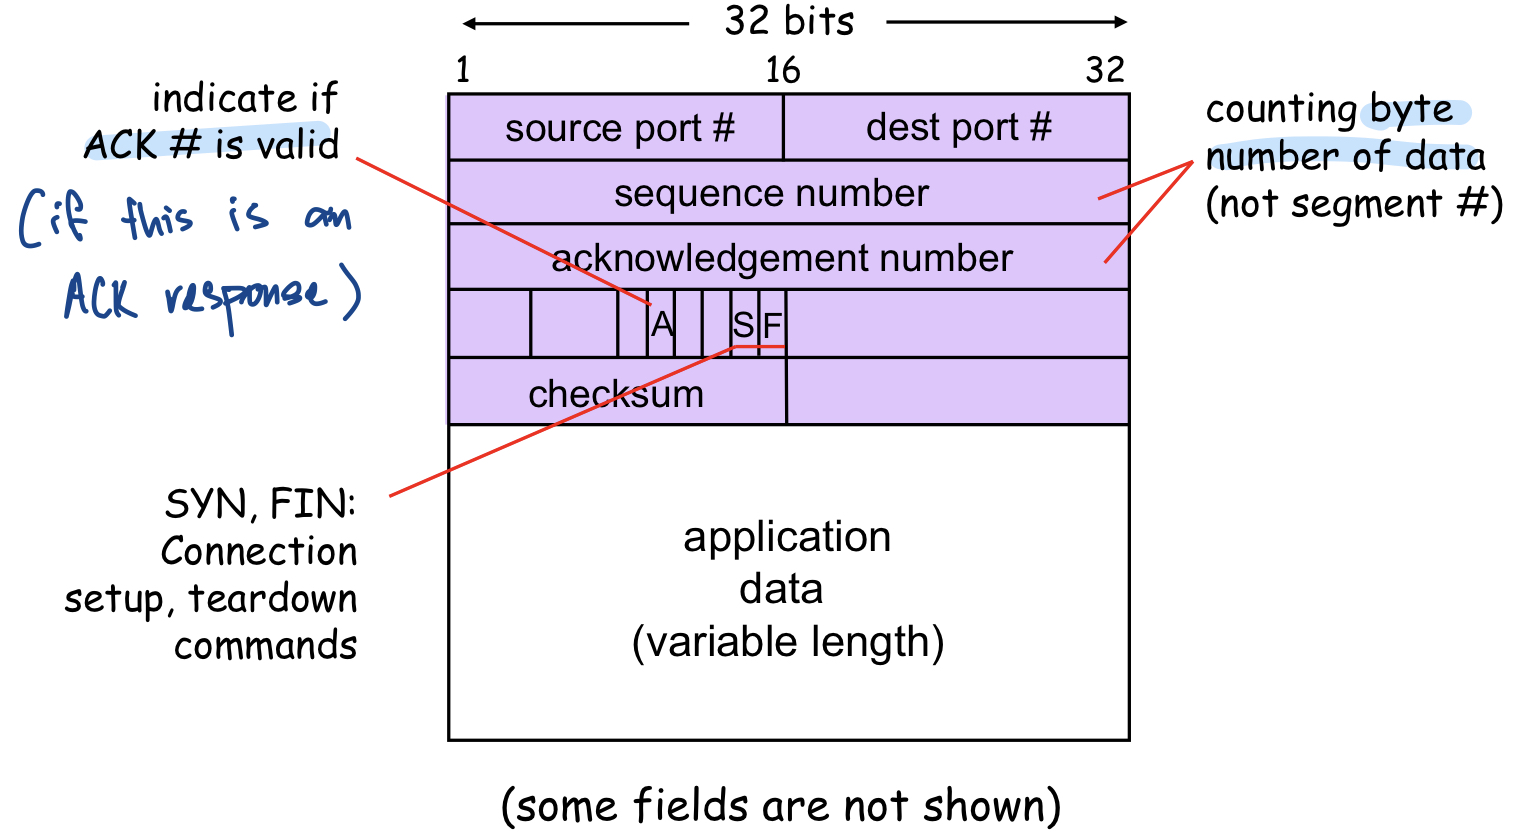
\includegraphics[scale=.14]{./assets/tcpHeader}\\

		Sequence Number:\\
		\blue{Byte number} of the \blue{first} byte of data in a segment\\

		ACK (cumulative):\\
		TCP ACKs up to the first missing byte in the stream (next expected byte number)\\
		Eg. If segment is [0-999], receiver would ACK 1000\\
		\highlight{NOTE:} TCP does not specify how receiver should handle \blue{out of order} segments, it is up to implementer.\\

		TCP Sender Events\\
		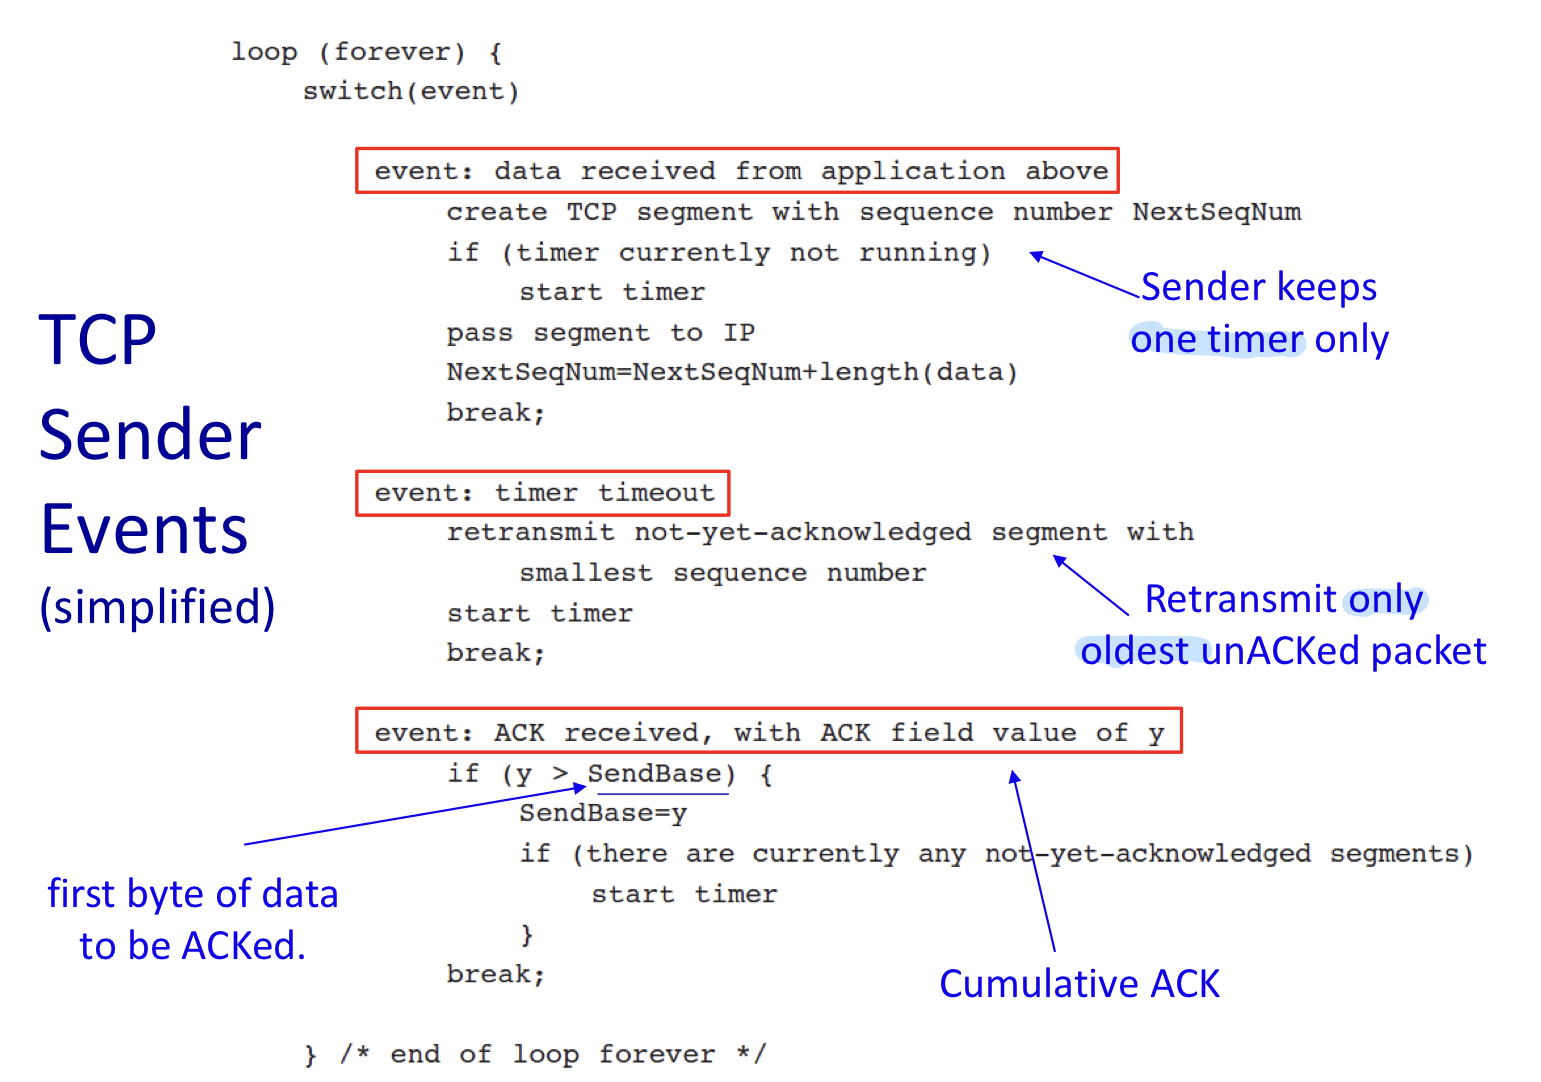
\includegraphics[scale=.17]{./assets/tcpSenderEvents}

		TCP Receiver Events\\
		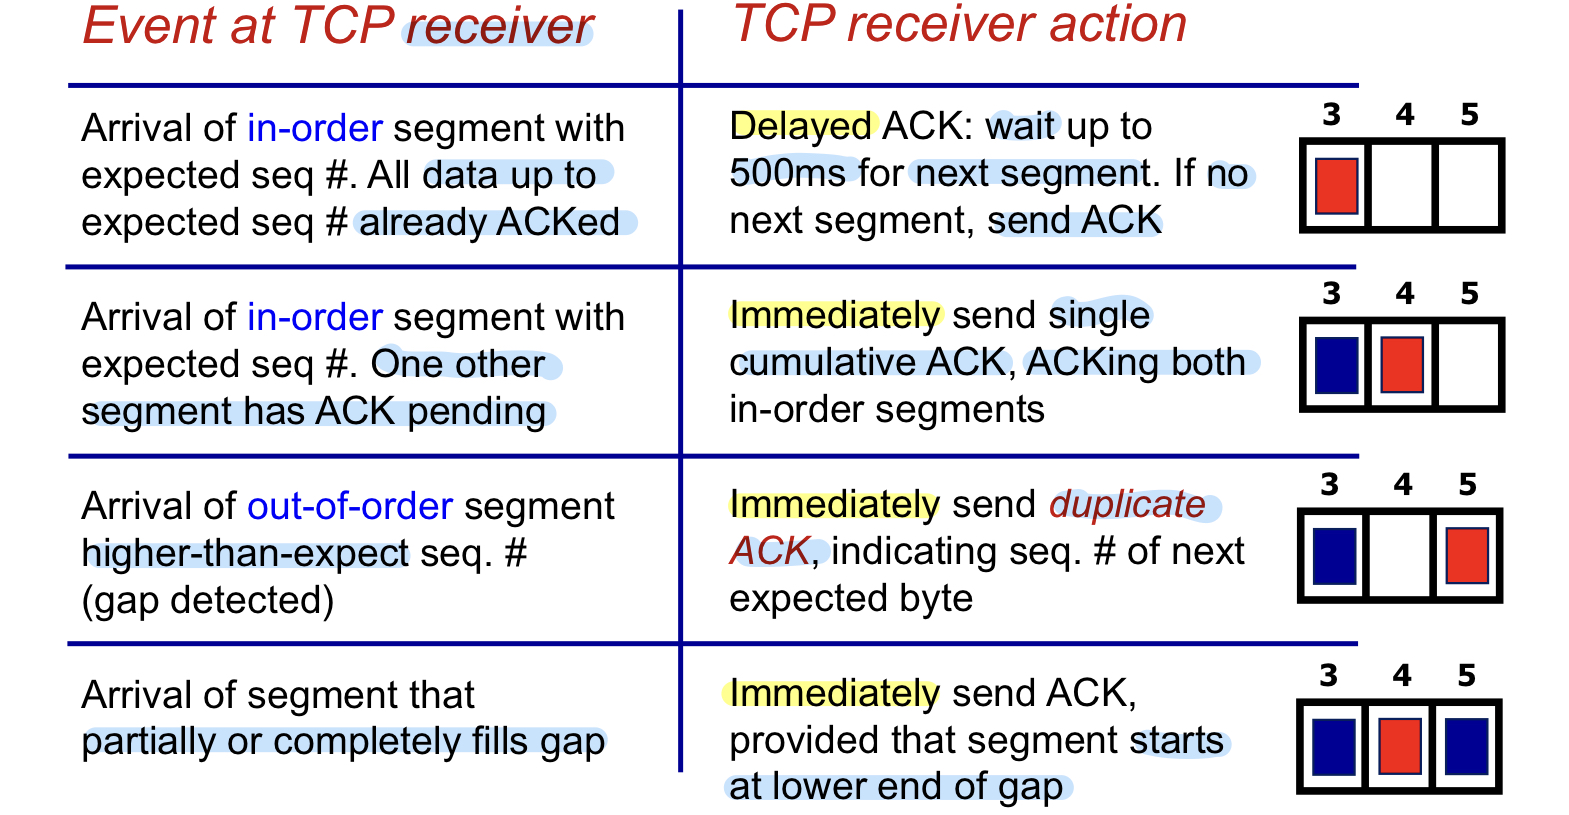
\includegraphics[scale=.15]{./assets/tcpReceiverEvents}

		TCP Fast Retransmission\\
		If sender receives \blue{4 duplicate ACKs} (ACK for the same segment), it supposes the segment is lost.\\
		Immediately resend segment, even before timer expires\\

		Establishing connection - 3-way Handshaking\\
		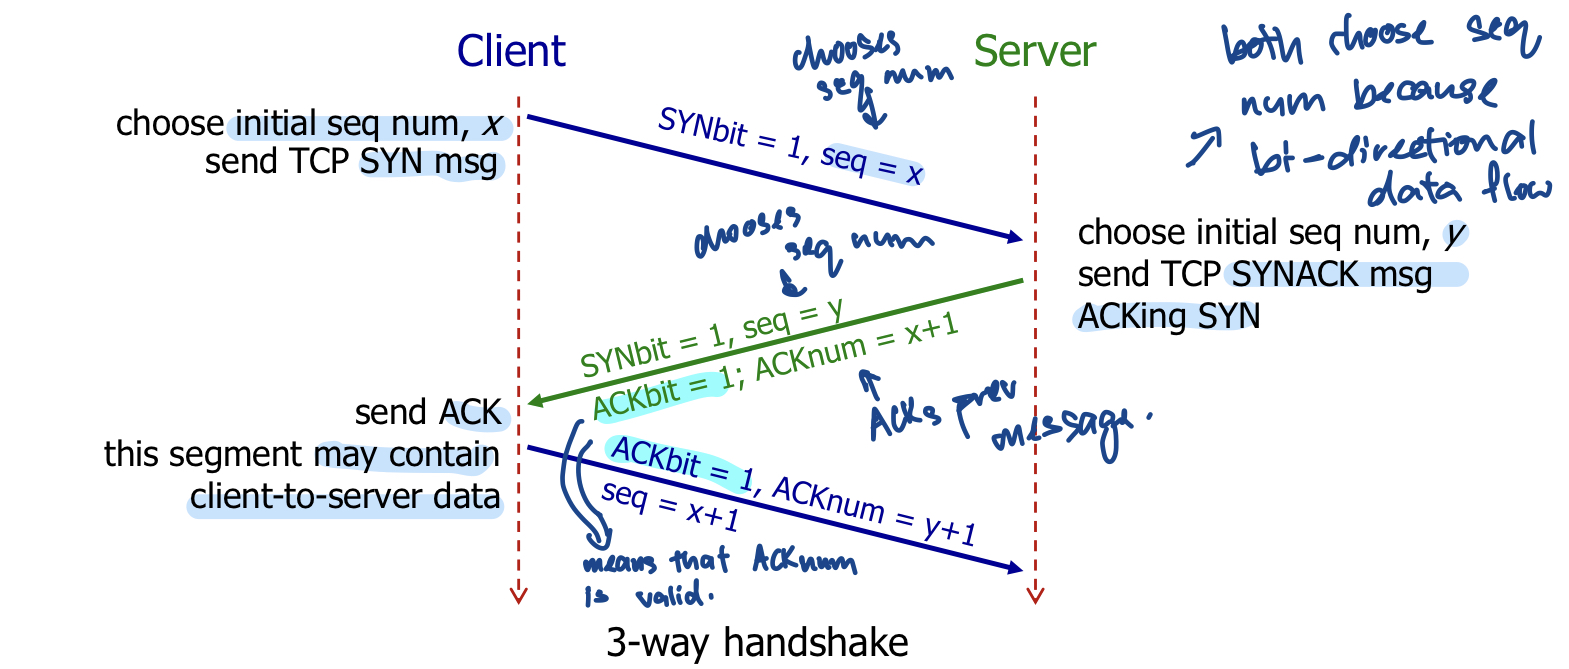
\includegraphics[scale=.15]{./assets/tcpHandshaking}

		Closing Connection\\
		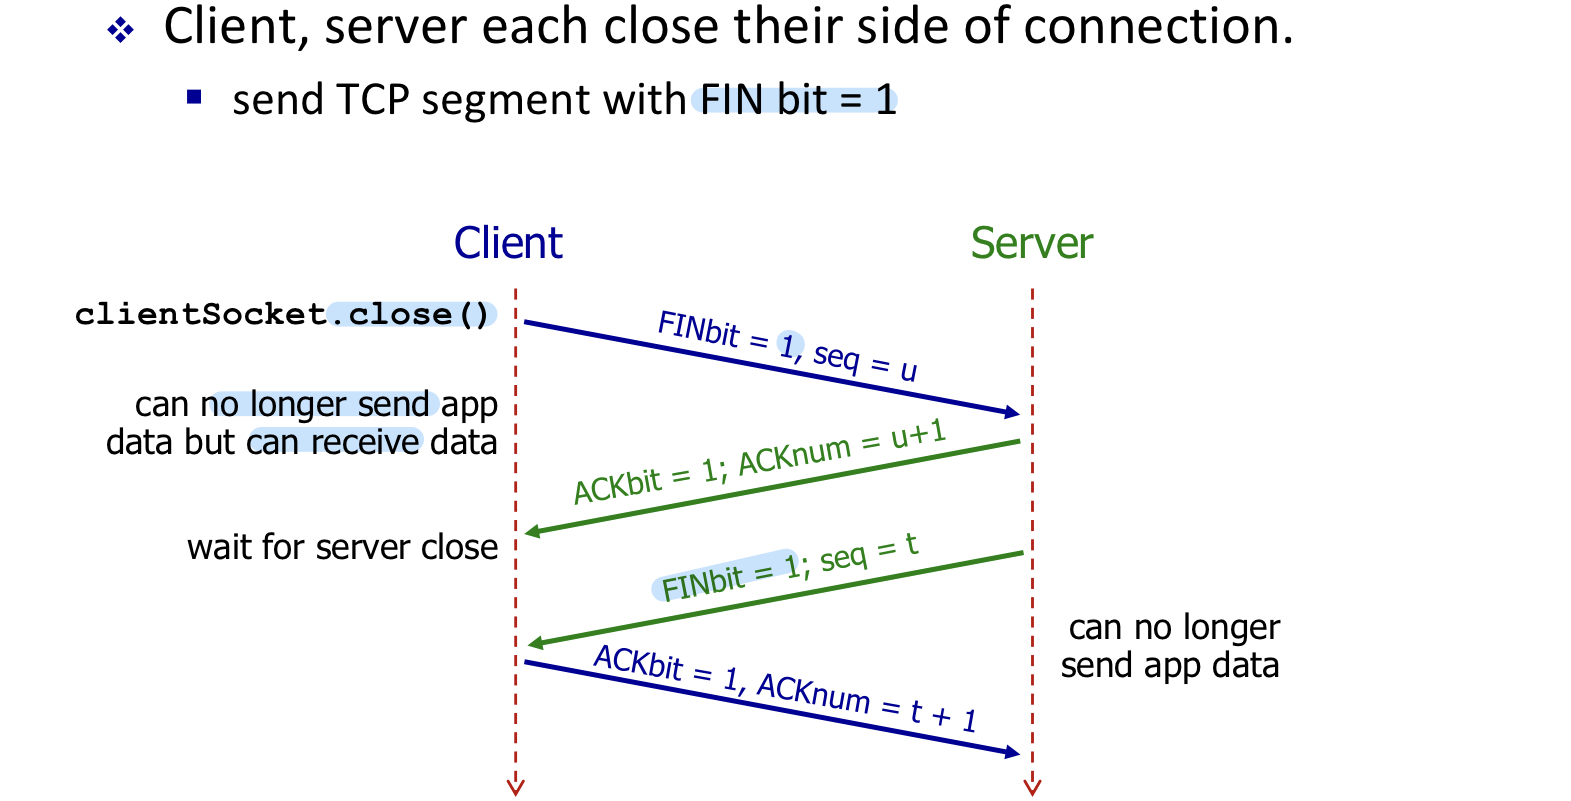
\includegraphics[scale=.14]{./assets/tcpCloseConnection}

		{\normalsize\textbf{Network Layer}}\\
		host to host\\

		\textbf{IP Address}\\
		IP Address is used to identify a host or router\\
		32-bit integer expressed in either binary or decimal\\
		Hosts get IP addresses via:\\
		1. Manual configuration by system administrator\\
		2. Automatically assigned by Dynamic Host Configuration Protocol (DHCP) server\\
		DHCP is more scalable\\
		\highlight{NOTE:} IP addresses are associated with a \blue{network interface}\\
		- each network interface has its own IP, eg laptop with ethernet port and wifi will have 2 IP addresses\\
		- routers typically have many interfaces\\
		\textbf{DHCP}\\
		Allows a host to dynamically obtain its IP address from DHCP server when it joins network\\
		- IP addr is renewable\\
		- allows reuse of IP addresses\\
		- supports mobile users joining network\\

		\blue{4 step process:}\\
		1. Host boradcasts \blue{``DHCP discover''} message\\
		2. DHCP server responds with \blue{``DHCP offer''} message (note that a host may get more than 1 offer)\\
		3. Host requests IP addr with \blue{``DHCP request''} message\\
		4. DHCP server sends address with \blue{``DHCP ACK''} message\\

		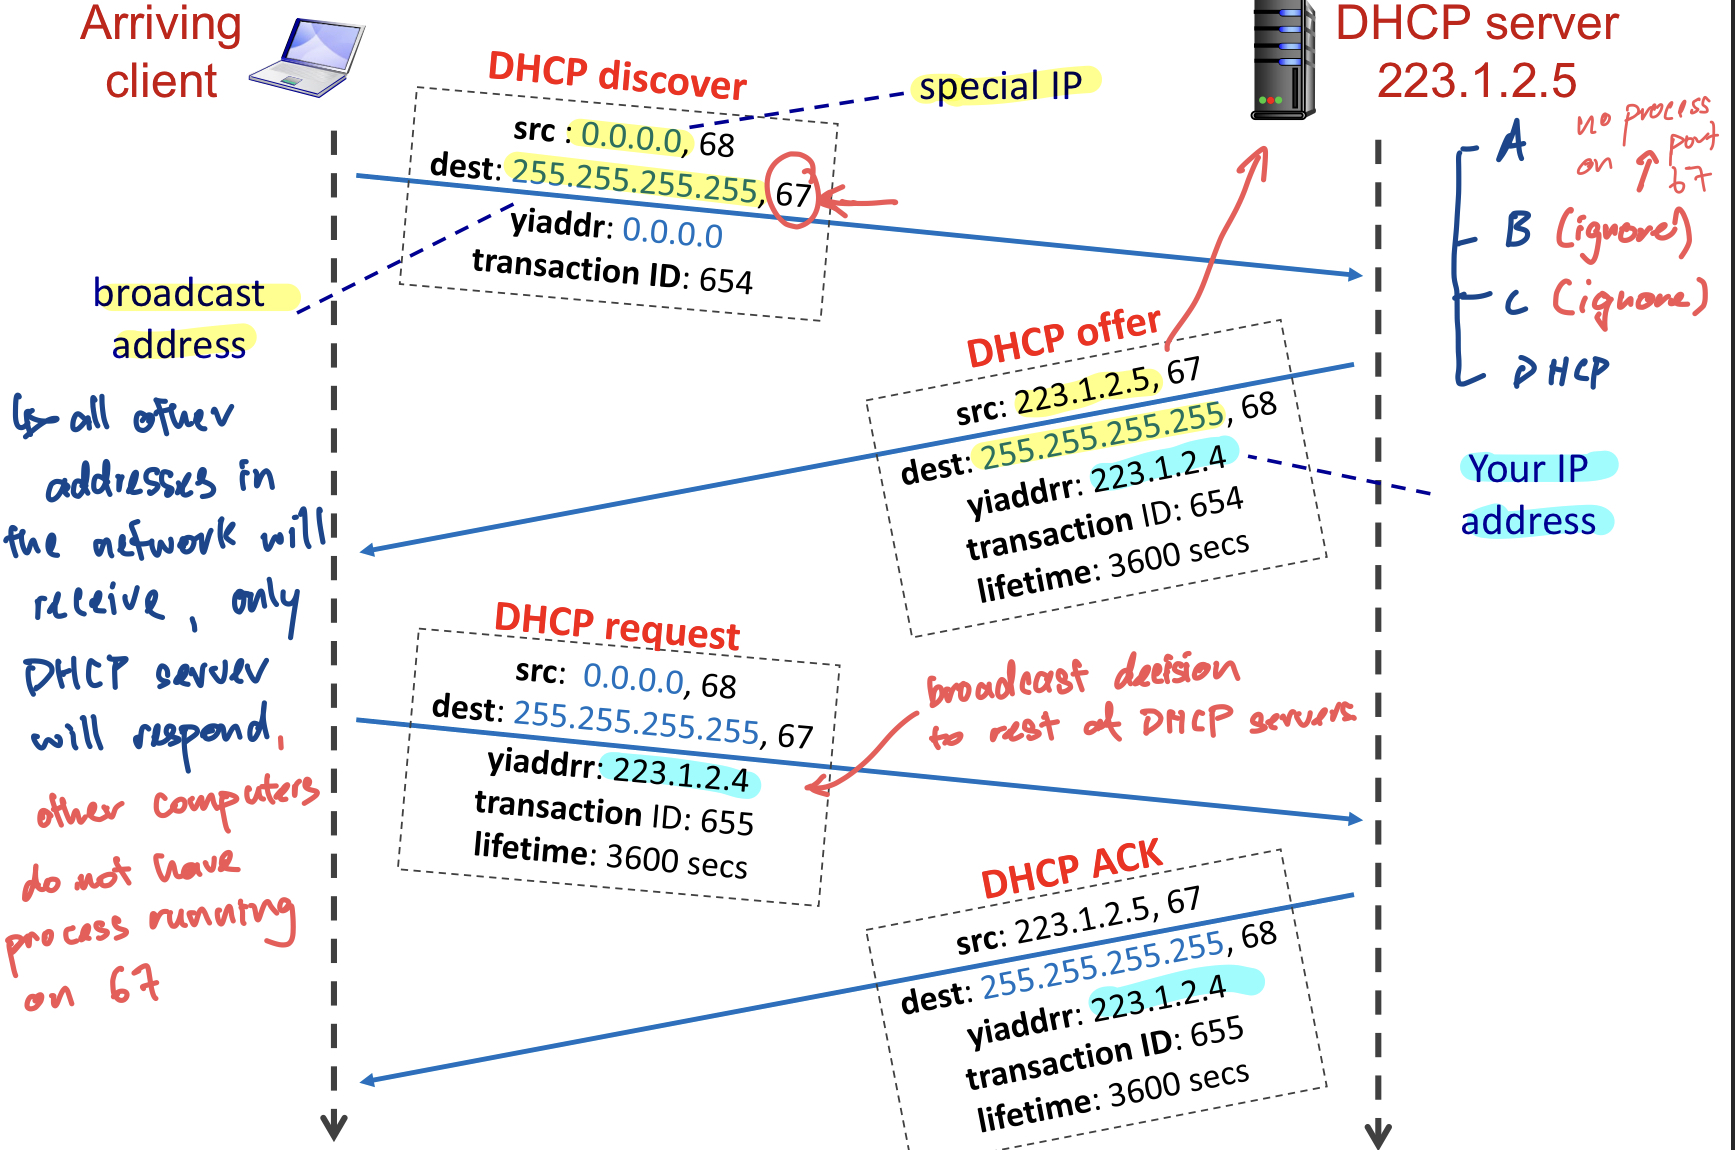
\includegraphics[scale=.15]{./assets/dhcp}
		\red{NOTE:} DHCP may also provide additional network information\\
		- IP address of \blue{first-hop router} (default gateway)\\
		- IP address of \blue{local DNS server}\\
		- \blue{Network mask}\\
		\red{NOTE:} DHCP runs over UDP, server on port 67, client port 68\\

		Special IP Addresses\\
		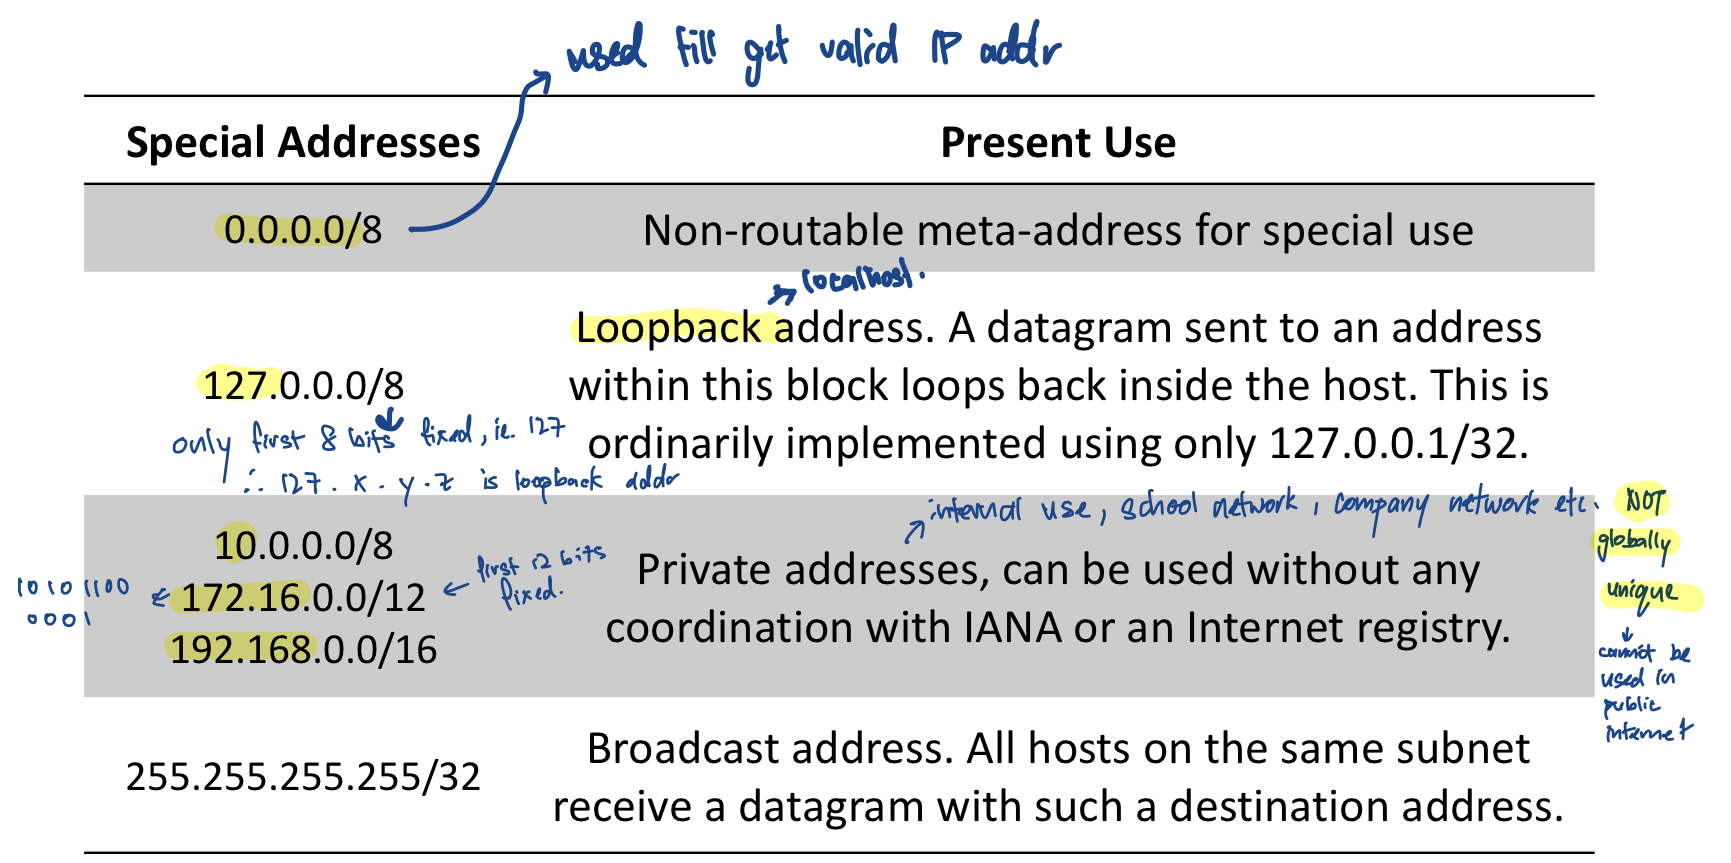
\includegraphics[scale=.16]{./assets/specialIpAddr}

		\textbf{Subnets}\\
		IP addresses comprises of two parts:\\
		1. network (subnet) prefix\\
		2. host ID\\
		\red{Subnet} is a network formed by a group of ``directly'' interconnected hosts\\
		- hosts in the same subnet have the same network prefix\\
		- hosts in the same subnet can physically reach each other \blue{without intervening router}\\
		- They connect to the outside world through a router\\

		\textbf{CIDR}\\
		Classless Inter-domain Routing is the Internet's IP address assignment strategy\\
		- subnet prefix is of arbitrary length\\
		- address format: \highlight{a.b.c.d/x}, where x is the number of bits in subnet prefix\\

		\textbf{Subnet Mask}\\
		\red{Subnet Mask} is used to determine which subnet an IP address belongs to\\
		- Made by setting all subnet prefix bits to 1s and host ID bits to 0s\\
		\texttt{and} with IP address to get subnet prefix\\

		\textbf{Hierarchical Addressing}\\
		Allows efficient advertisement of routing information\\
		- instead of having a routing table with $2^{32}$ entries, use block allocations\\
		- Eg. A router could broadcast ``send me anything with addresses beginning with 200.23.16.0/20''\\
		Can have smaller and more efficient routing tables\\
		\highlight{NOTE:} These are not subnet masks/ prefixes!!\\
		Routers use \highlight{longest prefix match} to determine where to route to\\

		\textbf{Routing Algorithms - Intra AS routing}\\
		- AS: Autonomous System\\
		- View network as a graph of nodes (routers) and edges (links)\\
		- Each link can have an associated cost eg. money, congestion, avail bandwidth etc.\\
		\red{Goal:} find least cost path between two vertices in graph\\

		\textbf{``link state'' algorithms}\\
		- All routers have complete knowledge of network topology and link cost; Routers periodically broadcast link costs to each other\\
		- Use Djikstra's Algo to compute least path (using this global map)\\

		\textbf{``distance vector'' algorithms}\\
		- Routers know physically-connected neighbours and link costs to neighbours\\
		- Routers \blue{exchange} local views with neighbours and update own local views based on neighbours'\\
		- Iterative process of computation: Swap local view with neighbours, update own local view, repeat until no change\\
		- \blue{Key Difference:} Only broadcast link costs to immediate neighbours\\

		Graph Notations:\\
		- $c(x, y)$: cost of link between routers $x, y$, $\infty$ if not direct neighbours\\
		- $d(x, y)$: cost of least-cost path between routers $x, y$\\

		\textbf{Bellman-Ford Equation}\\
		\centerline{$d_{x}(y) = min_{v}{c(x, y) + d_{v}(y)}$}\\
		where min is taken over all direct neighbours $v$ of $x$\\

		Intuitively, shortest path from x to y is the minimum of least cost to each neighbour of x + least cost path from neighbour to y\\
		- To find the least cost path, x needs to know the cost from each of its direct neighbours to y\\
		- Each neighbour v sends its \blue{distance vector (y, k)} to x, telling x that the cost from v to y is k\\

		Algorithm Steps\\
		1. Every router \textbf{x, y, z} sends its distance vectors to its directly connected neighbours.\\
		2. When x finds out that y is advertising a path to z that is cheaper than x currently knows, x will\\
		\tab 2.1 \blue{update its distance vector to z} accordingly\\
		\tab 2.2 note that \blue{all packets for z should be sent to y}. This info is used to create x's forwarding table\\
		3. After several rounds, all routers know least-cost paths to all other routers\\

		\textbf{Routing Information Protocol (RIP)}\\
		- RIP implements DV algo, using \blue{hop count} as cost metric (insensitive to network congestion)\\
		- Exchange routing table every 30 seconds over \blue{UDP port 520}\\
		- ``self-repair'': is no update from a neighbour router for 3 mins, assume neighbour has failed, remove neighbour entry from table\\

		\textbf{Network Address Translation (NAT)}\\
		Public IP: unique, $2^{32}$ addresses, many are reserved\\
		Private IP: used within a network, \red{NOT} globally unique, ie. can't be used outside network\\

		\textbf{NAT router}\\
		NAT routers sit between a local network and wider internet\\
		- \blue{Replace} (src IP addr, port no.) of \red{every outgoing datagram} to (NAT IP addr, new port no.)\\
		- \blue{Remember} in NAT translation table, the mapping from (src IP addr, port no.) to (NAT IP addr, new port no.)\\
		- \blue{Replace} (NAT IP addr, new port no.) in dest fields of every \blue{incoming datagram} with corresponding (src IP addr, port no.) stored in NAT translation table\\
		\green{Effect:} \red{all} datagrams \red{leaving} local network have the same src NAT IP addr (new port no. are not the same)\\

		\textbf{Benefits of using NAT}\\
		- No need to rent a range of public IP addr from ISP; just one for NAT router\\
		- All hosts use private IP addr. Can change address of hosts (within network) without notifying outside world\\
		- Can change ISP without changing addresses of hosts in local network\\
		- Hosts insde local network are not explicitly addressable and visible by outside world (security)\\

		\textbf{IPv4 Datagram Format}\\
		header size: 20 \blue{bytes}\\
		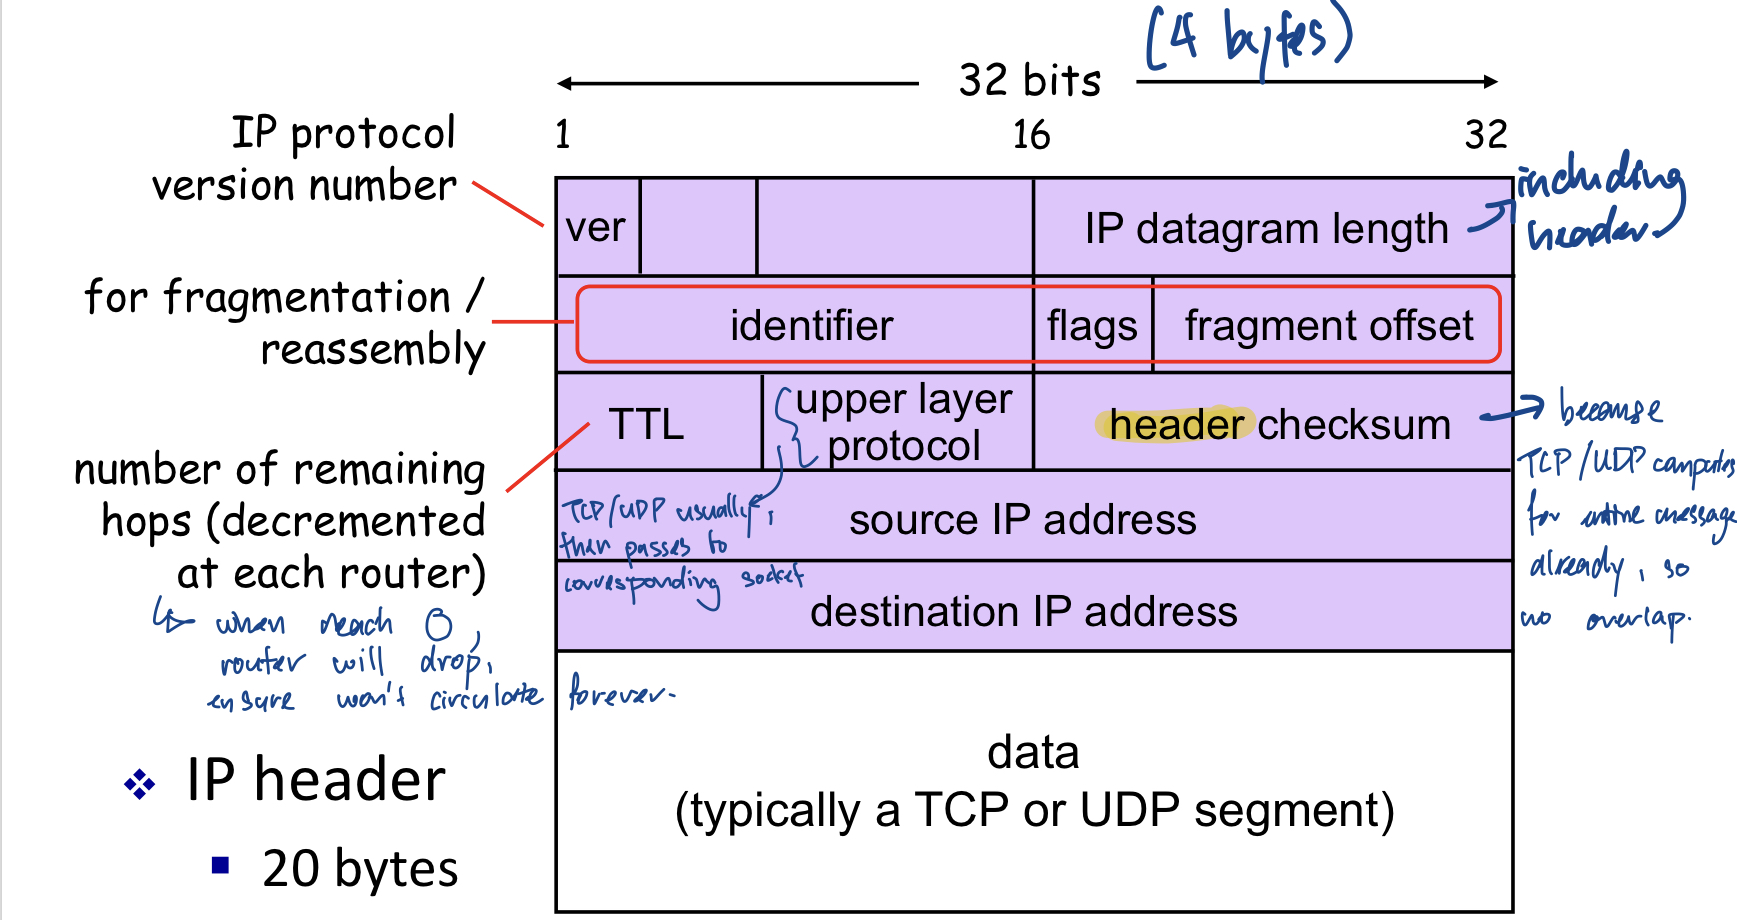
\includegraphics[scale=.14]{./assets/ipDatagram}

		\textbf{IP Fragmentation and Reassemby}\\
		- Different links may have different \blue{MTU} (Max Transfer Unit): max amount of data a link layer frame can carry (max size of IP datagram)\\
		- IP datagrams that are too large may be fragmented by router\\
		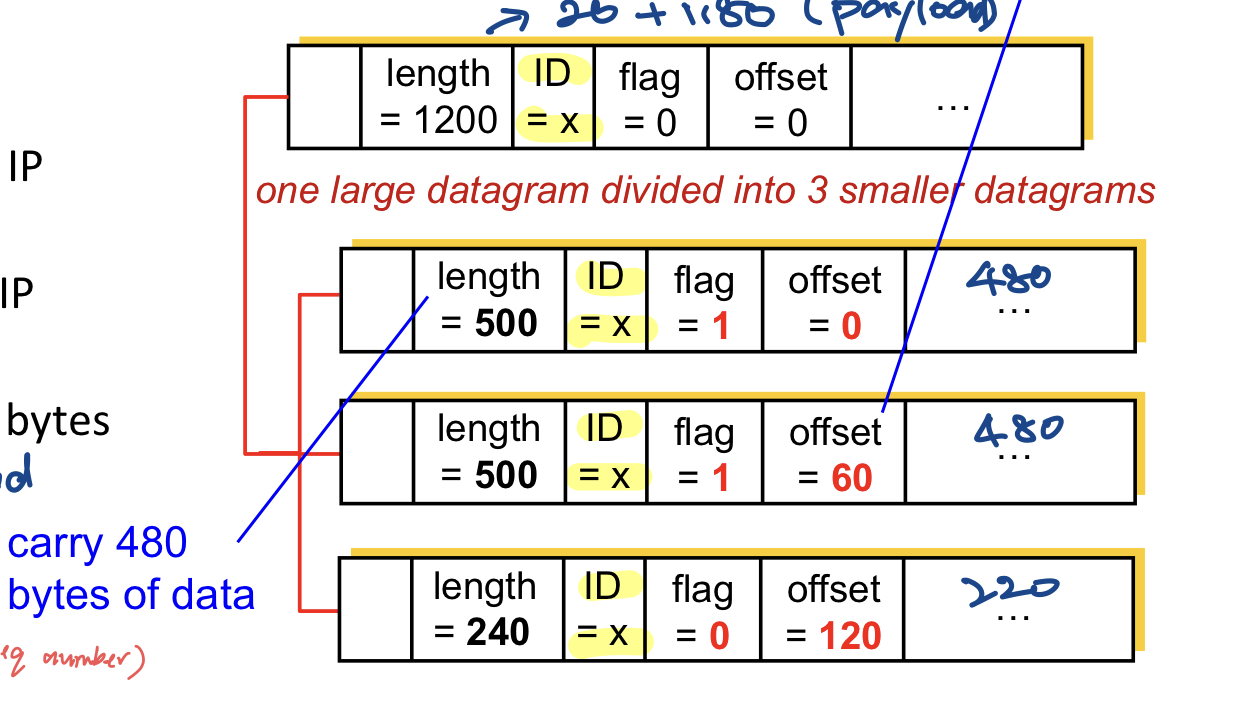
\includegraphics[scale=.15]{./assets/ipFragmentation}\\
		- Flag = 1 if there is next fragment in same segment, 0 if last fragment\\
		- Offset is expressed in units of \red{8-bytes}; first byte num / 8 (relative ordering between fragments)\\
		- ID remains the same for all fragments\\

		\textbf{Internet Control Message Protocol (ICMP)}\\
		Used by hosts and routers to communicate network-level info\\
		- Error reporting eg. unreachable host/ network/ port/ protocol\\
		- Echo request / reply (\texttt{ping})\\
		ICMP messages are carried in IP datagrams (ICMP header starts after IP header)\\
		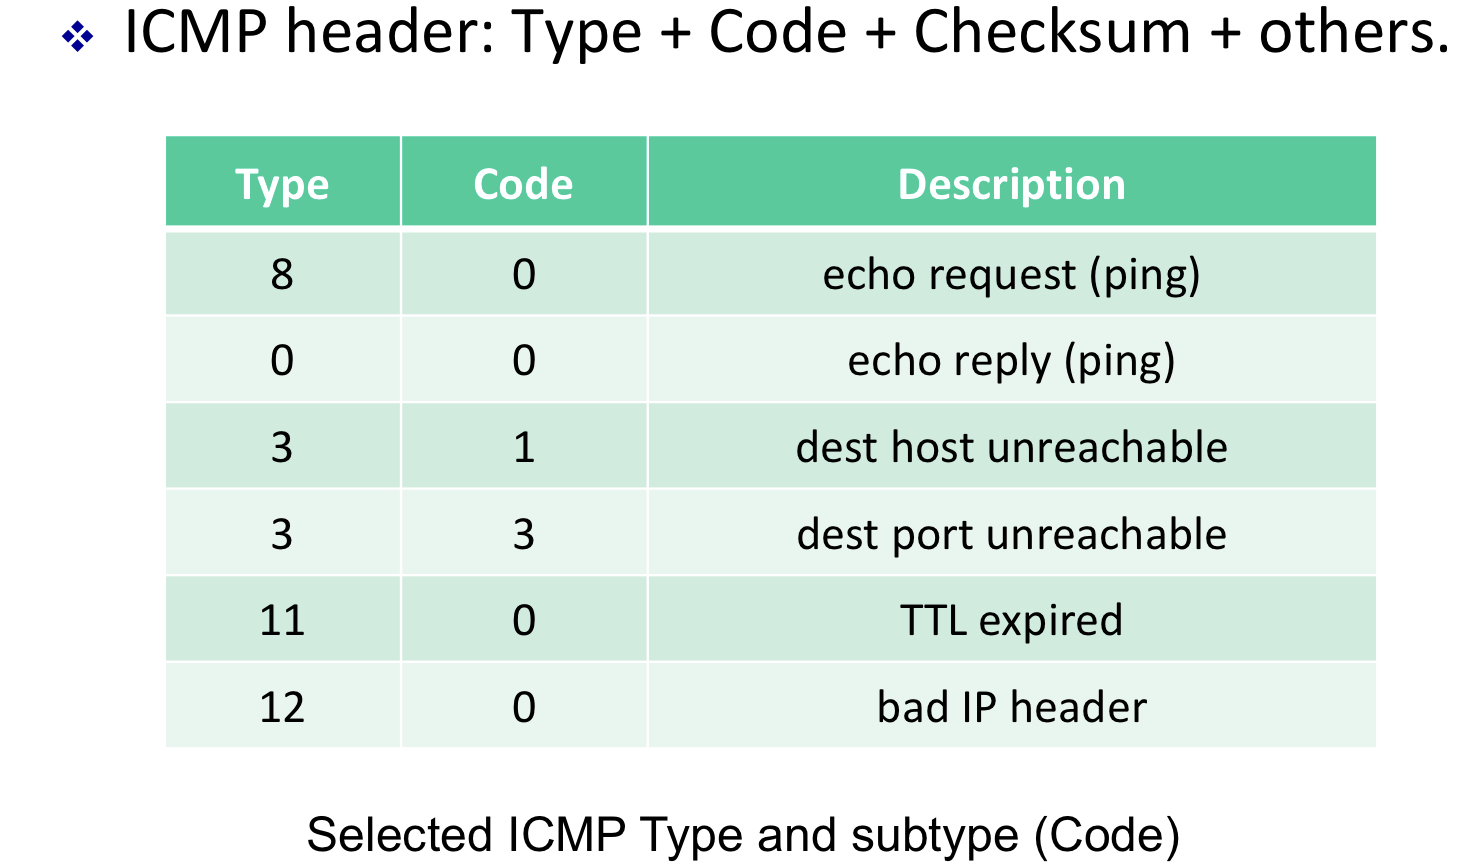
\includegraphics[scale=.14]{./assets/icmp}\\
		eg. TTL reaches 0, packet discarded, ICMP error message sent to datagram's src addr\\

		{\normalsize\textbf{Link Layer}}\\
		Sending datagrams between adjacent nodes (single link)\\
		IP datagrams encapsulated in link layer frame for transmission\\
		Implemented in adapter (NIC) or chip, adapters are semi-autonomous, implementing link and physical layers\\

		\textbf{Link Layer Services (protocols may not implement all)}\\
		- \blue{Framing}: encapsulate datagram in fram (adding header, trailer)\\
		- \blue{Link access control}: coordinate which node can send frames and when, when multiple nodes share common link\\
		- \blue{Reliable delivery}: seldom on low bit error link (fibre) but used on error-prone link (wireless)\\
		- \blue{Error detection}\\
		- \blue{Error correction}: identifies and corrects bit errors without retransmission\\

		\textbf{Error Detection and Correction}\\
		Link Layer uses mainly \blue{Parity Checking} and \blue{CRC} (CRC is good but slow in software $\rightarrow$ not used in TCP/UDP/IP)\\
		Error detection schemes are not 100\% reliable\\

		Parity Checking\\
		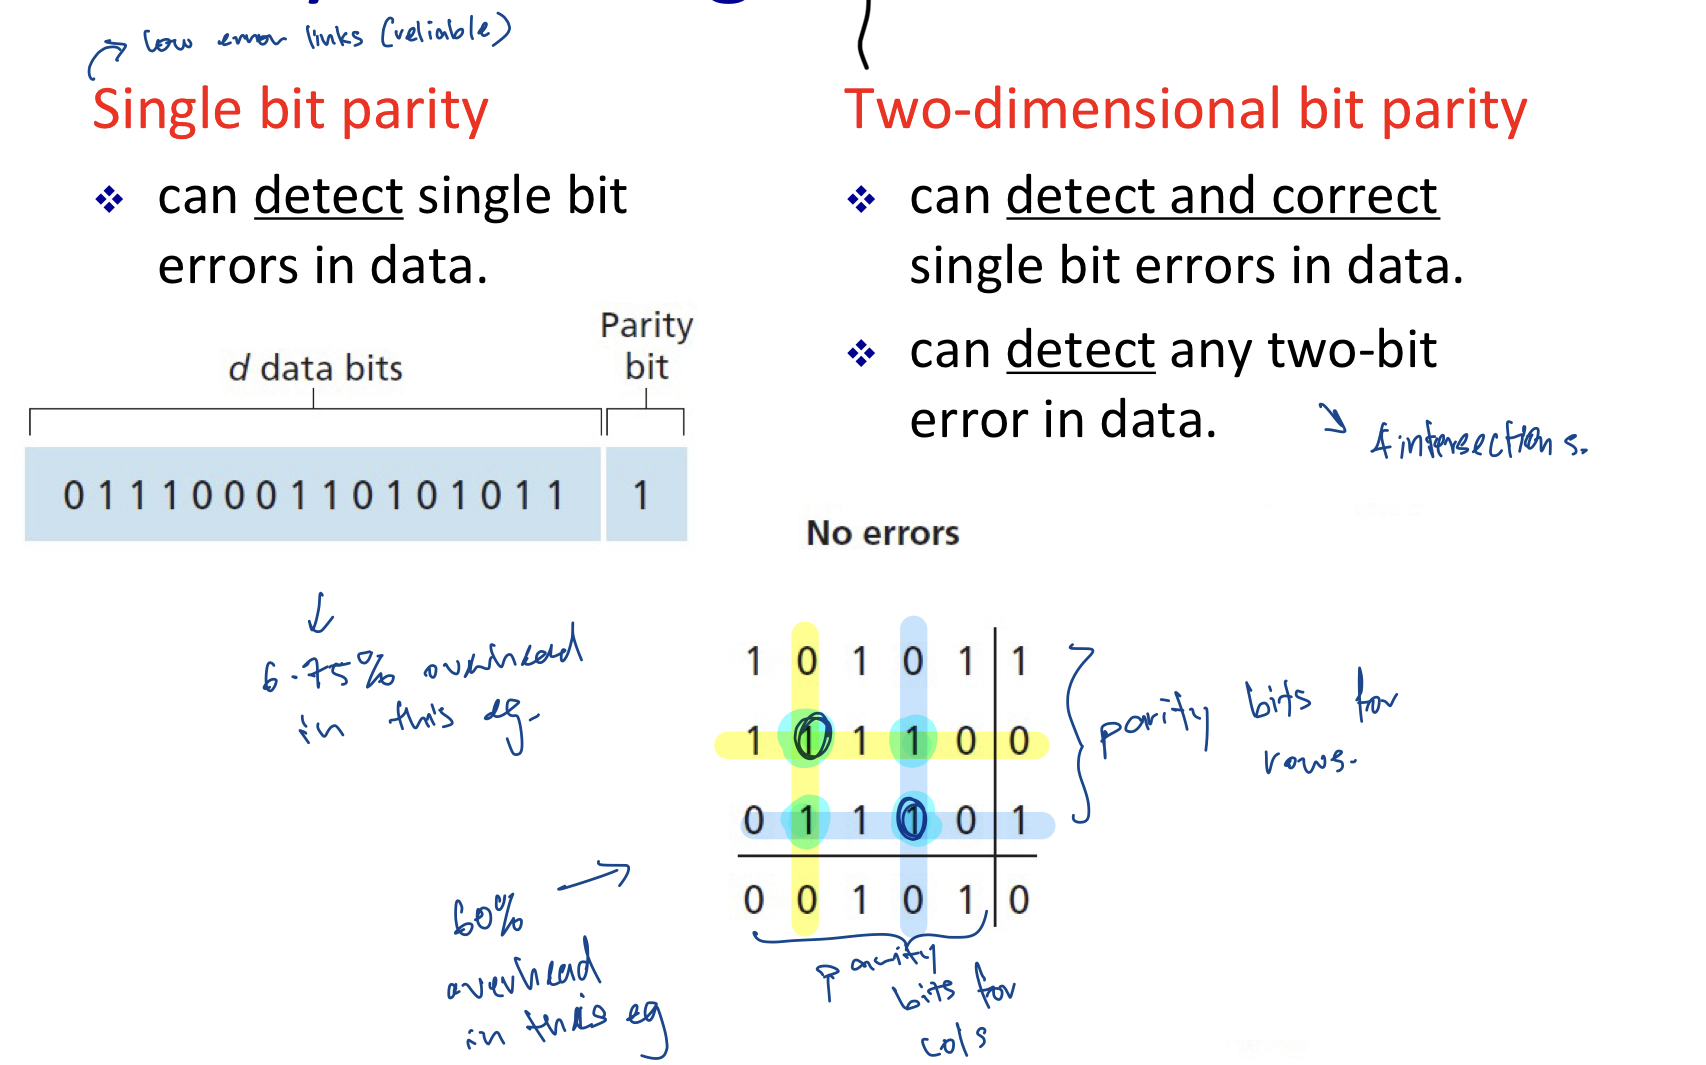
\includegraphics[scale=.15]{./assets/parityChecking}

		Cyclic Redundancy Check (CRC)\\
		Bitwise \texttt{xor} operation without carry or borrow\\
		- \red{D}: data bits, viewed as a binary number\\
		- \red{G}: generator of $r + 1$ bits, agreed by sender and receiver beforehand\\
		- \red{R}: will generate CRC of $r$ bits\\
		Sender sends (D, R)\\
		Receiver knows G, divides (D, R) by G $\rightarrow$ if non sero remainder, \red{error!}\\
		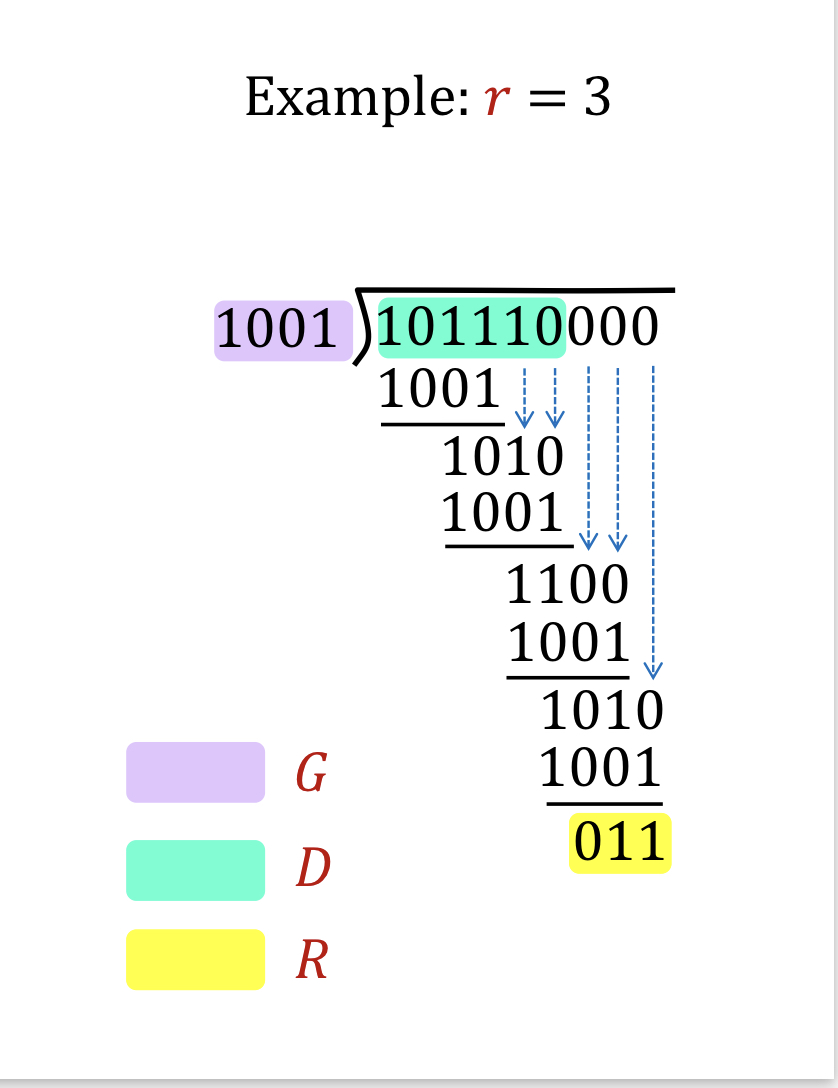
\includegraphics[scale=.13]{./assets/crc}

		\textbf{Type of Network Links}\\
		1. Point to point link: sender and receiver connected by a dedicated link (or switch with star topology)\\
		2. Broadcast link (shared medium): multiple notes connected to a shared broadcast channel, when a node transmits a frame all other notes receives a copy (wifi, satellite, ethernet with bus topology)\\

		\textbf{Mulitple Access Protocols}\\
		In broadcast channel, if two or more nodes transmit simultaneously\\
		- every node receives multiple frames at the same time $\rightarrow$ frames \blue{collide} at nodes and none would be correctly read\\

		\red{Multiple Access Protocols}\\
		- distributed algorithm that determines how nodes share channel, ie. when a node can transmit\\
		- However, coordination about channel sharing must use channel itself (no out of band channel signalling)\\

		Types of Multiple Access Protocols\\
		\red{Channel partitioning}\\
		- divide channel into fixed smaller ``pieces'' (time slots, frequency)\\
		- allocate piece to node for exclusive use\\
		- \red{Cons:} wastage, partitions must be divided beforehand (hard to add new hosts)\\
		- \green{Pros:} Good if all have equal amount of data to send\\
		\red{Taking turns}\\
		- nodes take turns to transmit\\
		\red{Random Access}\\
		- Channel is not divided, collisions possible\\
		- Need to recover from collisions\\

		\textbf{Channel Partitioning}\\
		Time Division Multiple Access (TDMA)\\
		- Access to channel in ``rounds''\\
		- Each node gets fixed length (frame transmission time) slot in each round\\
		- \blue{Unused slots go idle}\\

		Frequency Division Multiple Access (FDMA)\\
		- Channel Spectrum is divided into frequency bands\\
		- Each node is assigned a fixed frequency band\\
		- Unused transmission time in frequency bands go idle\\

		\textbf{Taking Turns}\\
		Polling\\
		- master node ``invites'' slave nodes to transmit in turn\\
		- Concerns: polling overhead (not huge), single point of failure (master node)\\
		- Need to be able to detect if master node fails, and choose new master\\

		Token Passing\\
		- Control token is passed from one node to next sequentially\\
		- Concerns: token overhead, single point of failure (token)\\
		- node with token may fail, need algo to generate exactly 1 token\\

		\textbf{Random Access}\\
		- No prior coordination between nodes on when to transmit\\
		- two or more transmitting nodes $\rightarrow$ \red{collision}\\
		Protocols specify:\\
		- how to detect collisions\\
		- how to recover from collisions\\

		Slotted ALOHA\\
		\blue{Assumptions}\\
		- All frames are of equal size\\
		- Time is divided into slots of equal length (time to transmit 1 frame)\\
		- Nodes start to transmit only at the beginning of a slot\\

		\blue{Operations}\\
		- Listens to channel while transmitting (collision detection)\\
		- \red{if collision happens:} node \blue{retransmits} a frame in each \blue{subsequent slot} with probability \red{p} until success\\
		\red{p} is recalculated frequently to take into account things like congestion etc. \\
		perfect p: 37\%\\

		Pure ALOHA\\
		No slots, no synchronisation\\
		- When there is a fresh frame: transmit immediately\\
		- Chance of collision increases: frame sent at $t_{0}$ collides with other frames sent in $(t_{0}-1, t_{0} + 1)$\\
		Rude in the sense that a node may start transmitting while another node is already transmitting (better protocol below)\\
		16\% max utilisation\\

		\textbf{Carrier Sense Multiple Access (CSMA)}\\
		Sense the channel before transmission, if \green{idle} transmit, if \red{busy}, defer transmission\\
		- Main idea is not to interrupt others\\
		But \red{collisions} may still exist\\
		- when two nodes transmit simultaneously\\
		- before one detects the other has started due to propagation delay\\
		Even after detect collision, node still continues to finish transmission of frame, then retransmit later (waste of time)\\

		\textbf{CSMA/CD (collision detection)}\\
		- Same as CSMA except that when collision is detected, transmission is \blue{aborted immediately} (reduces channel wastage)\\
		- Retransmit after \blue{random} amount of time\\
		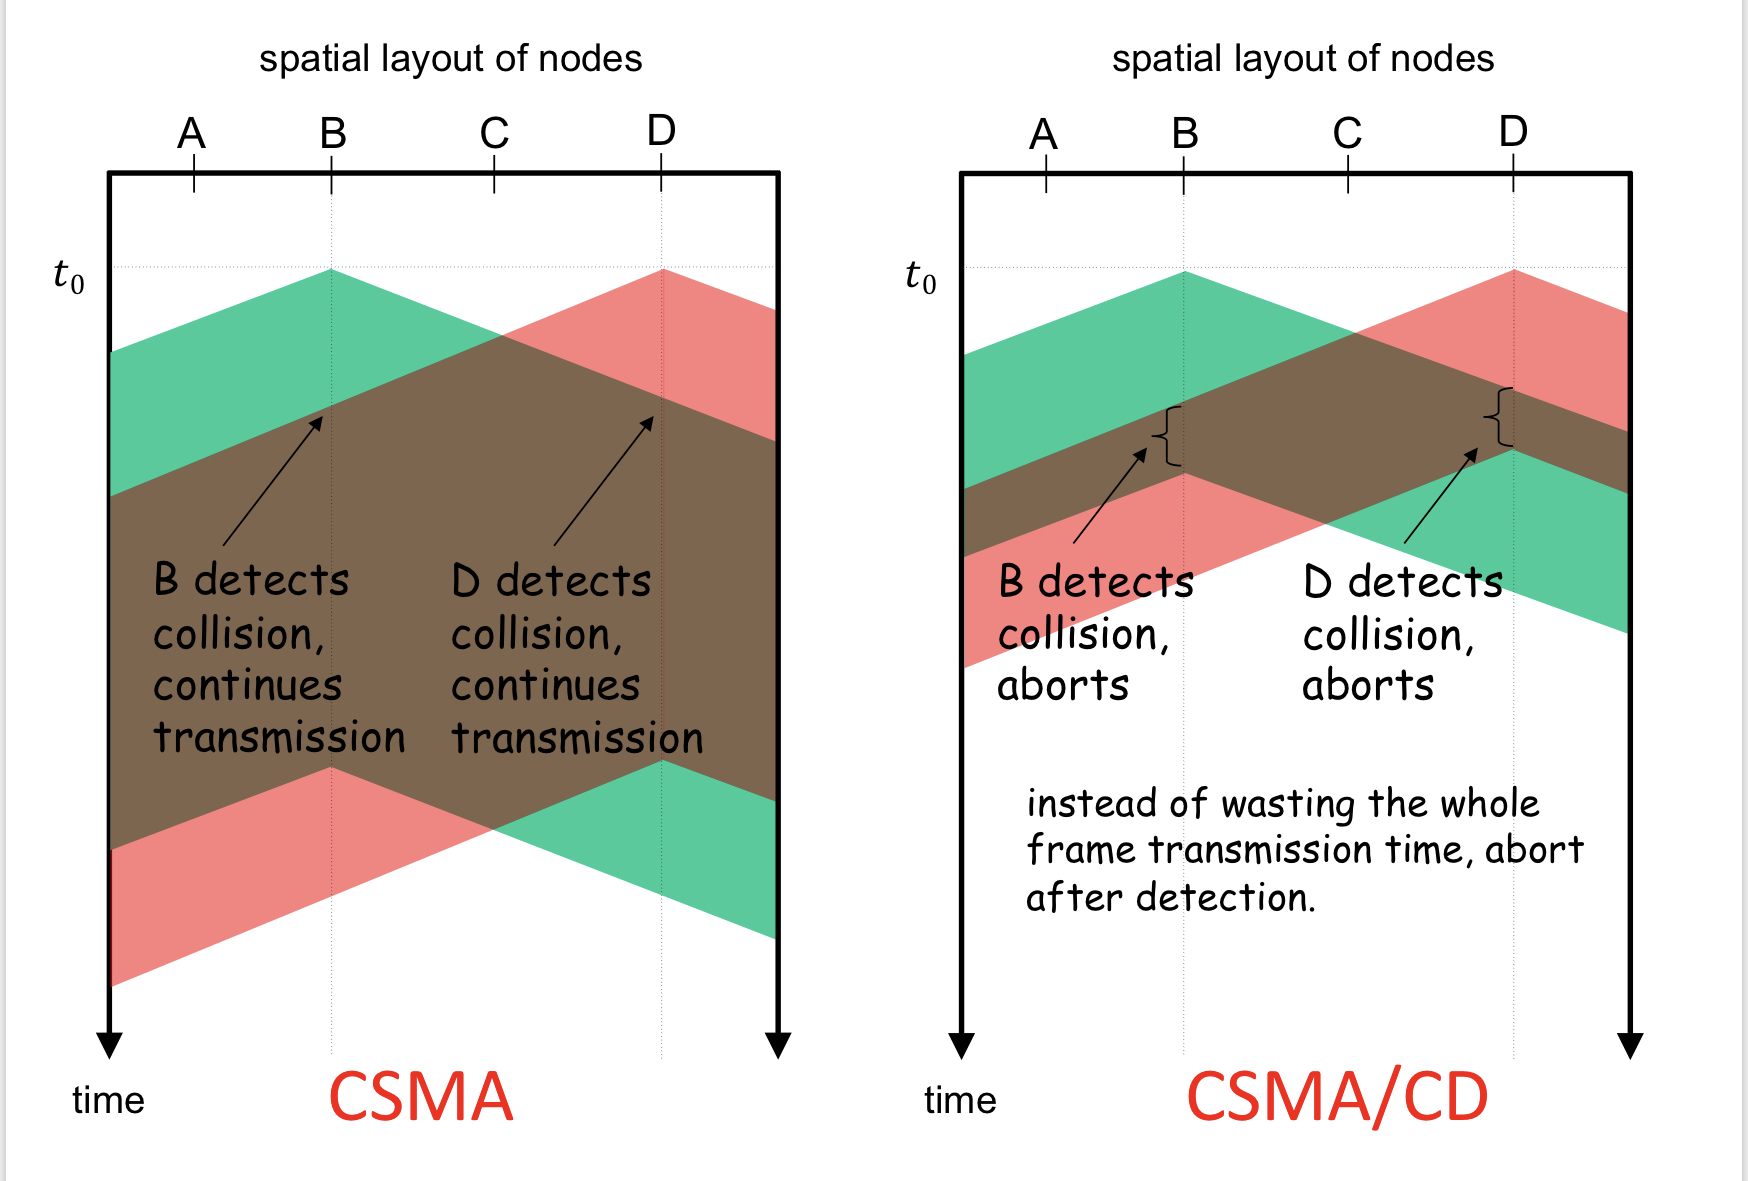
\includegraphics[scale=.13]{./assets/CSMA}\\

		Minimum Frame Size\\
		if frame size too small, \red{collision will still appear} but \red{may not be detected} by sending nodes (no retransmission)\\
		Eg. Ethernet requires min. frame size of 64 Bytes\\
		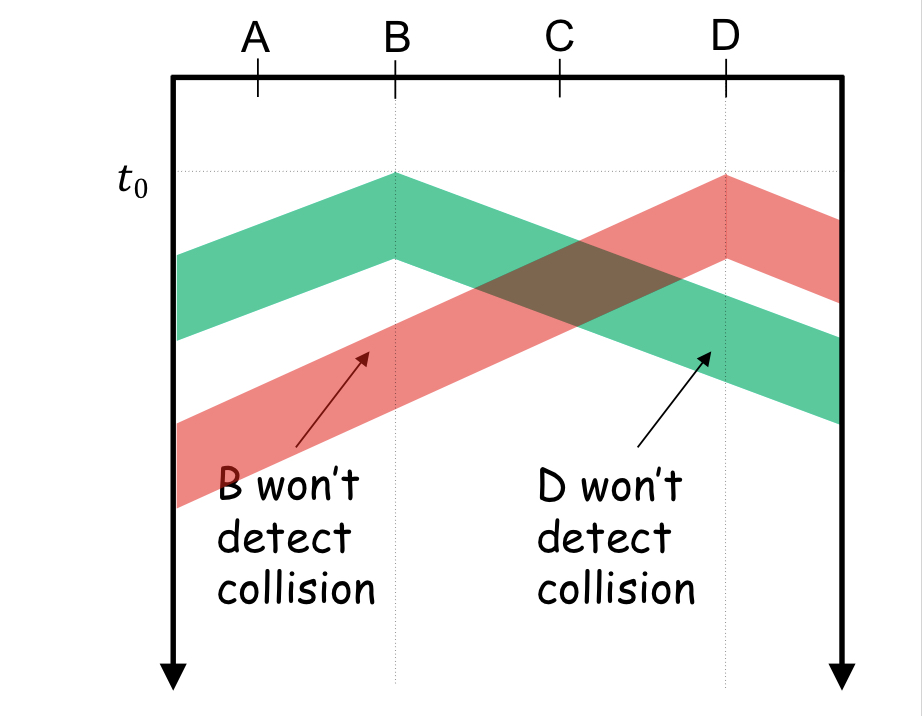
\includegraphics[scale=.14]{./assets/csmaMinFrame}

		\textbf{CSMA/CA (Collision Avoidance)}\\
		Collision detection easy in wired LAN (10V instead of 5V), but difficult in wireless\\
		Hidden Node Problem:\\
		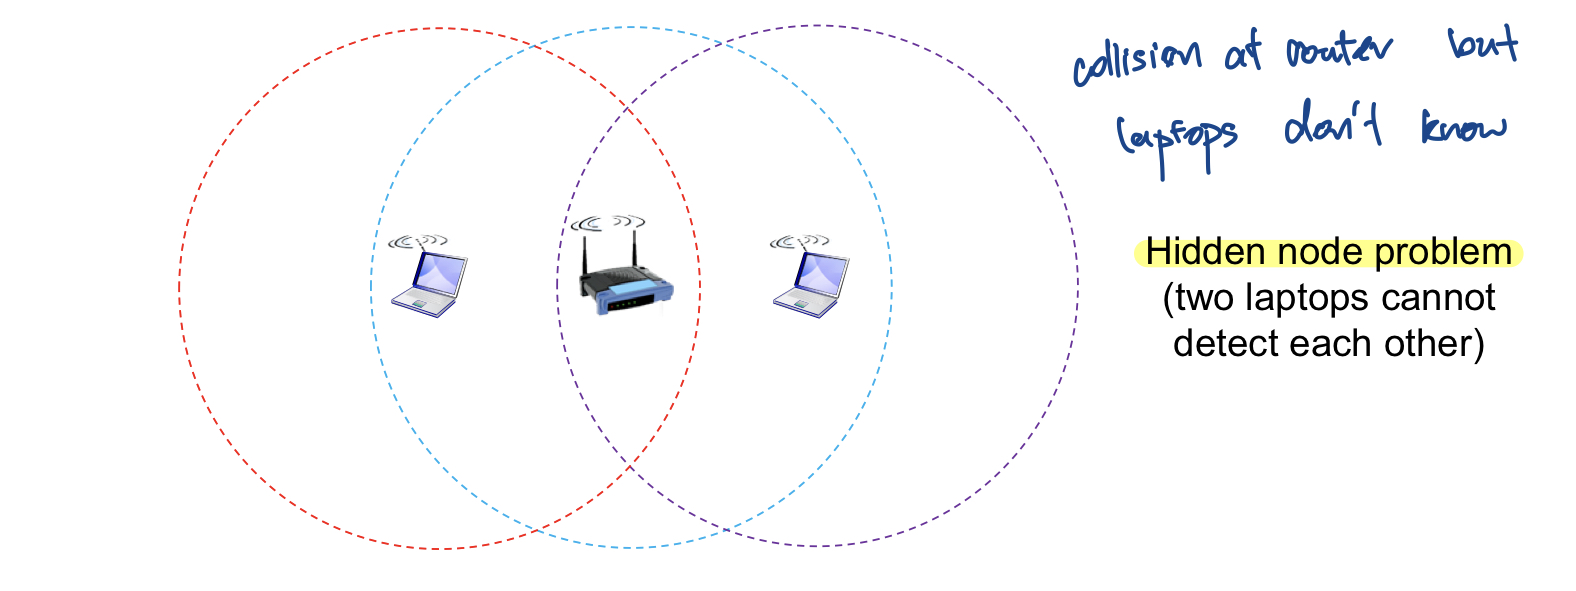
\includegraphics[scale=.15]{./assets/hiddenNode}\\
		In CSMA/CA, receiver returns ACK if frame received OK\\

		\red{NOTE: }Switches are \blue{peer-transparent}, just a way of connecting hosts, doesn't manipulate frames going through them\\

		\textbf{MAC Address}\\
		- Every adapter (NIC) has a \blue{MAC Address} (Media Access Control)\\
		- MAC address is used to send and receive link layer frames.\\
		\tab - When adapter recieves frame, check if dest MAC matches its own\\
		\tab\tab - if \red{yes}: extract datagram and passes to protocol stack\\
		\tab\tab - if \red{no}: discard frame without interrupting host\\
		This check is done very fast without disturbing the CPU\\
		\red{NOTE:} IP identifies host, MAC identifies NIC\\

		- Every MAC Address is \blue{gloablly unique}, typically \blue{hardcoded (burned)} into NIC ROM, typically \blue{48 bits}

		\textbf{MAC Address vs IP Address}\\
		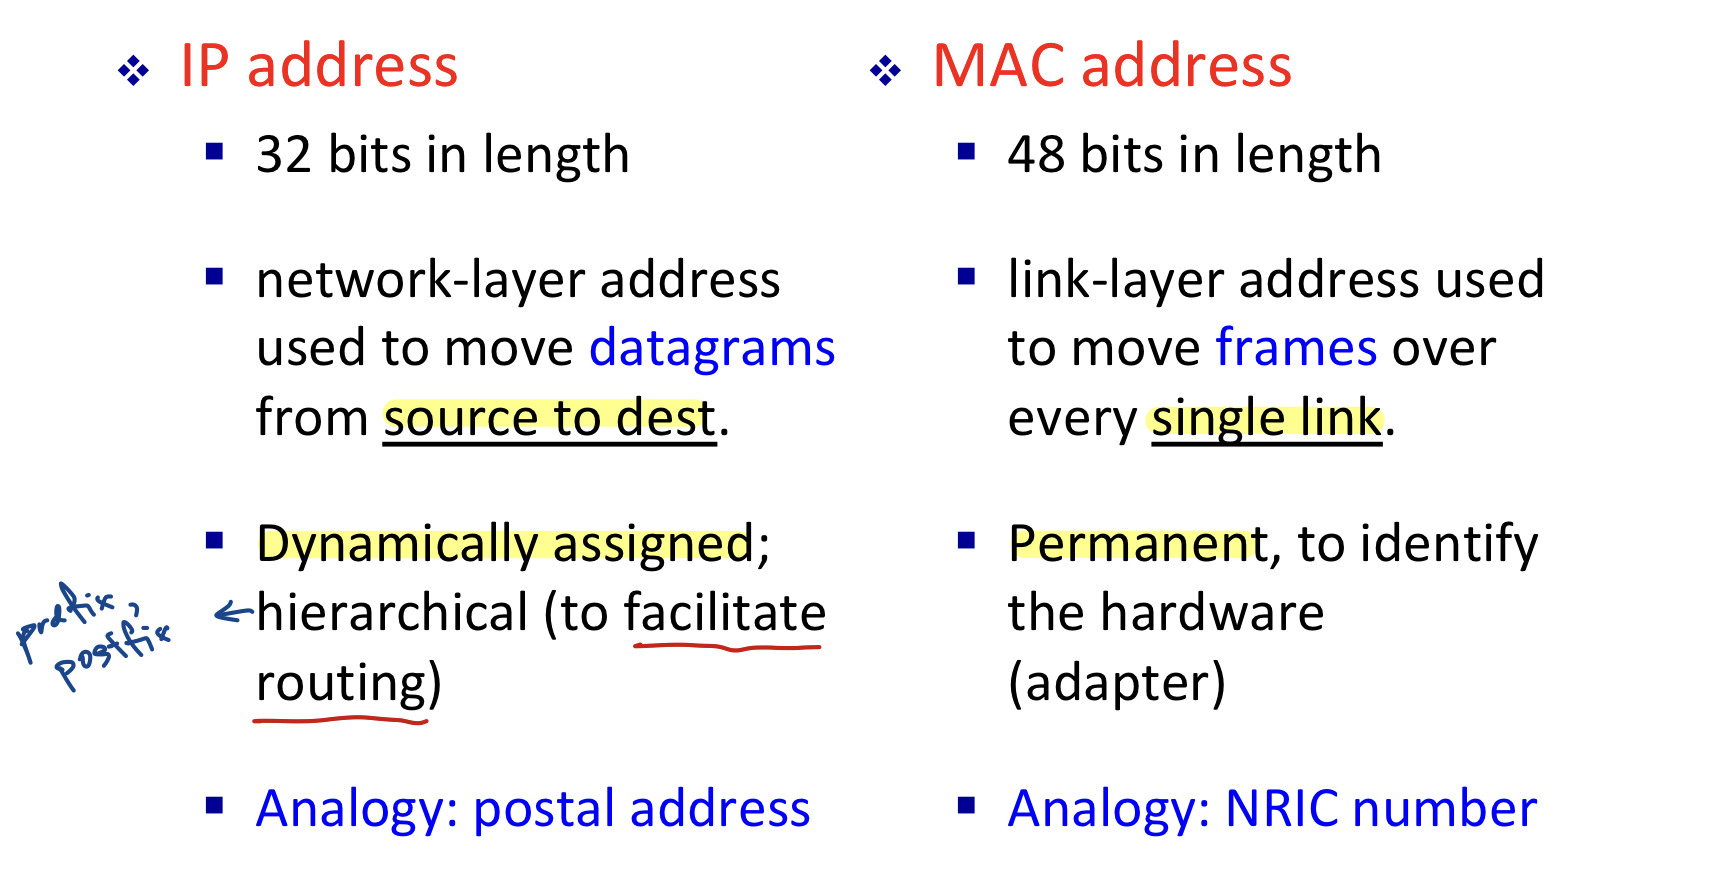
\includegraphics[scale=.13]{./assets/macVsIp}\\

		\textbf{Address Resolution Protocol (ARP)}\\
		To get MAC address of receiving host, knowing its IP (using DNS or otherwise)\\
		- Each node (host / router) has an \blue{ARP table}\\
		- ARP table stores the mappings of IP address and MAC address of other nodes in the \red{same subnet}\\
		- Only stores nodes that it had communications with, not all nodes in subnet
		- Each entry consists of \red{IP addr, MAC addr, TTL}\\

		\textbf{Sending a frame in the same subnet (A$\rightarrow$B)}\\
		If A knows B's MAC addr (from ARP table)\\
		\tab 1 Create a frame with B's MAC addr and send\\
		\tab 2 \red{Only B} will process this frame\\
		\tab 3 Other nodes may receive but ignore this frame\\
		If A does not know B's MAC Addr\\
		\tab 1 A \red{broadcasts ARP query packet} with B's \blue{IP addr}\\
		\tab\tab 1.1 Dest MAC addr = FF-FF-FF-FF-FF-FF\\
		\tab\tab 1.2 All other nodes in subnet will receive but only B will reply\\
		\tab 2 B replies to A with its MAC Addr\\
		\tab\tab 2.1 Pass up to network layer to check IP addr\\
		\tab\tab 2.2 Replay frame is sent to A's MAC address (included in query packet)\\
		\tab 3 A adds B's IP-to-MAC mapping in ARP table (until TTL expires)\\
		\highlight{NOTE:} Determine if B is in same subnet by checking network mask + network prefix\\
		\highlight{NOTE:} Get B IP addr via DNS\\
















		

		
		
	\end{multicols*}
\end{document}
